

%!TEX root = /Users/sbogutzky/Entwicklung/projects/bogutzky/repositories/2939413/final-draft.tex
\section{Flow und Gehen (intraindividuell)} 

% (fold)
\label{sec:flow_und_gehen_intraindividuell}

\subsection{Einleitung} 

% (fold)
\label{sub:einleitung_5_2}

Im Kontext des \acs{BMBF}-Projekts entwickelte Barbara Grüter die Hypothese, dass die kardio-lokomotorischen Phasensynchronisation als implizites Merkmal des (Flow-) Erlebens beim Gehen zu verwenden ist. In der in diesem Abschnitt beschriebenen Machbarkeitsstudie überprüften wir diese Hypothese in Zusammenarbeit mit Licinio Roque und Rui Craveirinha (beide von der Universität Coimbra, Portugal). Im Aufbau glich diese Machbarkeitsstudie der in Abschnitt~\ref{sec:flow_und_laufen_intraindividuell} beschriebenen Laufstudie. 

% subsection einleitung (end)
\subsection{Methode} 

% (fold)
\label{sub:methode_5_2}

Die gesamte Machbarkeitsstudie bestand aus sechs Sitzungen mit sechs Gängen und einer Zeitdauer von etwa 1,25 Stunden. Die Untersuchungsperson ging für etwa eine Stunde und füllte alle 15 Minuten eine \ac{FKS} auf dem Smartphone aus. Zur Beantwortung der \ac{FKS} gab ich keine Hilfestellung. Die Termine verteilte wir auf sechs Wochentage in zwei aufeinanderfolgenden Wochen im Mai und Juni 2014. Der Start der Sitzungen variierte zwischen 11:45 Uhr und 13:00 Uhr. Die Gehstrecke war 5~km und ist in Abbildung~\ref{fig:landkarte_2} dargestellt.
\begin{figure}
	[!htb] \centering 
	\includegraphics[height=0.50 
	\textheight]{landkarte_1} \caption[Gehstrecke]{Gehstrecke -- Insgesamt 5~km (erstellt mit OpenStreetMap)} \label{fig:landkarte_2} 
\end{figure}

In dieser Machbarkeitsstudie ging eine gesunde Frau im Alter von 64 Jahren als zu untersuchende Person. Sie nutzte die Tätigkeit des Gehens, um den Kopf von ihrer beruflichen Tätigkeit frei zubekommen, Stress abzubauen sowie neue Inspirationen zu Themen ihrer Arbeit zu erhalten.

Ich rüstete sie vor jedem Lauf mit einem geladenen Smartphone, einem passenden Smartphone-Armband, zwei geladenen Shimmer \acp{IMU} mit Shimmer Gyro-Modulen, einem geladenen Shimmer \ac{IMU} mit Shimmer EKG-Modul sowie vier Einwegelektroden aus. Die Anordnung des Equipments ist der Abbildung~\ref{fig:equipment_2} zu entnehmen. Die Untersuchungsperson trug beim Gehen das Smartphone in dem passenden Smartphone-Armband am Oberarm, sofern sie es nicht zur Beantwortung einer \ac{FKS} nutzte. 
\begin{figure}
	[!htb] \centering 
	\includegraphics[width=1.00 
	\textwidth]{equipment_1} \caption[Equipment der Machbarkeitsstudie zum Flow-Erleben beim Gehen]{Equipment der Machbarkeitsstudie zum Flow-Erleben beim Gehen} \label{fig:equipment_2} 
\end{figure}

% subsection methode (end)
\subsection{Apparat} 

% (fold)
\label{sub:apparat_5_2}

In der beschriebenen Machbarkeitsstudie kam die gleiche Version des \ac{PPC}s und der \ac{PPP} zum Einsatz wie in der vorangegangenen Laufstudie. Ich ergänzte das Equipment um eine zweite Shimmer \ac{IMU} mit Gyro-Modul, die ich oberhalb der Hosentasche der Untersuchungsperson fixierte (siehe Abbildung~\ref{fig:equipment_2}). Die Aufnahme der Daten der zweiten Einheit diente zur Entwicklung einer Gangmerkmalerkennung, die für eine Smartphone App realisiert werden sollte, die auf zusätzliche \acp{IMU} verzichten kann (Abschnitt~\ref{sec:demonstrator}). Ich änderte die Sensorkonfiguration, da das Gehen eine geringe Abtastrate der Bewegung verlangt als das Laufen und weil eine zusätzliche \emph{Shimmer} \ac{IMU} mit Gyro-Modul das Datenaufkommen zusätzlich erhöht. Für eine höchstmögliche Auflösung des \ac{EKG}s testete ich die Abtastraten 512~Hz sowie 1024~Hz. Das Shimmer EKG-Modul ist in der Lage mit 1024~Hz abzutasten und die \ac{EKG}-Daten auf einen Flashspeicher zu sichern. Eine sofortige Bluetooth Übertragung ist aber nur bei 512~Hz gewährleistet. Die Konfiguration der beschriebenen Machbarkeitsstudie ist der Tabelle~\ref{tab:sensorkonfiguration_2} zu entnehmen.
\begin{table}
	[!htb] \caption[Sensorkonfiguration der Machbarkeitstudie zum Flow-Erleben beim Gehen]{Sensorkonfiguration der Machbarkeitstudie zum Flow-Erleben beim Gehen} \label{tab:sensorkonfiguration_2} \label{tab:sensorkonfiguration_fallstudie_gehen} 
	\begin{tabularx}
		{
		\textwidth}{p{.30
		\textwidth} p{.20
		\textwidth} p{.50
		\textwidth}} \toprule & Abtastrate & Betriebssicherer Messbereich \\
		\midrule EKG & 512~Hz & \\
		Beschleunigungsmesser & 56,7~Hz & 1,5~g \\
		Kreiselinstrument & 56,7~Hz & 500 $deg \cdot s^{-1}$ \\
		\bottomrule 
	\end{tabularx}
\end{table}

Die Berechnung der kardio-lokomotorischen Phasensynchronisation wurde zuerst durch Licinio Roque und Rui Craveirinha in Microsoft Excel realisiert und von mir in das in Abschnitt~\ref{sub:apparat_5_1} beschriebene R-Programm übertragen. 

% subsection apparat (end)
\subsection{Operationalisierung und gewonnene Daten} 

% (fold)
\label{sub:operationalisierung_und_gewonnene_daten_5_2}

Ich erhielt aus den sechs Sitzungen 23 Selbstauskünfte durch die Befragung mit der \ac{FKS}. Eine Selbstauskunft fehlt, weil die Untersuchungsperson versehentlich die App bei einer letzten Befragung schloss. Ich betrachtete die 23 Selbstauskünfte zur Verifizierung. Ich ermittelte den Mittelwert, die Standardabweichung jedes Items des Generalfaktors sowie der beiden Faktoren der \ac{FKS}. Für jeden Faktor und dessen Items berechnete ich die Item-Faktor-Korrelation (Tabellen~\ref{tab:generalfaktor_2}, \ref{tab:glatter_verlauf_2} und \ref{tab:absorbiertheit_2}). Daneben bestimmte ich für die Faktoren der \ac{FKS} die Maßzahl Cronbachs~$\alpha$. Die Item-Faktor-Korrelationen und die Reliabilität des Generalfaktors, des glatten Verlaufs und der Absorbiertheit mit Cronbachs~$\alpha$ = 0,98, 0,97 sowie 0,96 weisen auf eine gute Eignung hin. 

Zu jedem Befragungszeitpunkt gehören ca. 15 Minuten an \ac{EKG}-Daten und kinematischen Daten, die der \ac{PPC} vor jeder Befragung aufzeichnete. Es sind ca. 15 Minuten, da der Signalgeber nach 15 Minuten die Untersuchungsperson aufforderte, eine Selbstauskunft abzugeben. Das gewährleistete nicht in allen Fällen das Stehenbleiben und das Ausfüllen. Aus diesem Grund verwendete ich die Daten bis zum letzten erkannten Schritt vor der Fertigstellung des Fragebogens. Den letzten Schritt identifizierte ich im Nachhinein. 

Zur R-Spitzen-Erkennung nutzte ich die Ableitung II, da sie die größten R-Spitzen aufwieß. 

Ich berechnete einen mittleren normalisierten Shannon Entropie Index, um Zusammenhänge zwischen den expliziten Flow-Merkmalen der \ac{FKS} und kardio-lokomotorischen Phasensynchronisation zu untersuchen. Als Datengrundlage nutzte ich wieder die fünf Minuten an Daten direkt vor der Befragung mit der \ac{FKS}.

% subsection operationalisierung_und_gewonnene_daten (end)
\subsection{Ergebnisse} 

% (fold)
\label{sub:ergebnisse_5_2}

\subsubsection{Beobachtungen} 

% (fold)
\label{ssub:beobachtungen_5_2} 
\begin{figure}
	[!htb] % Created by tikzDevice version 0.10.1 on 2016-09-07 16:42:15
% !TEX encoding = UTF-8 Unicode
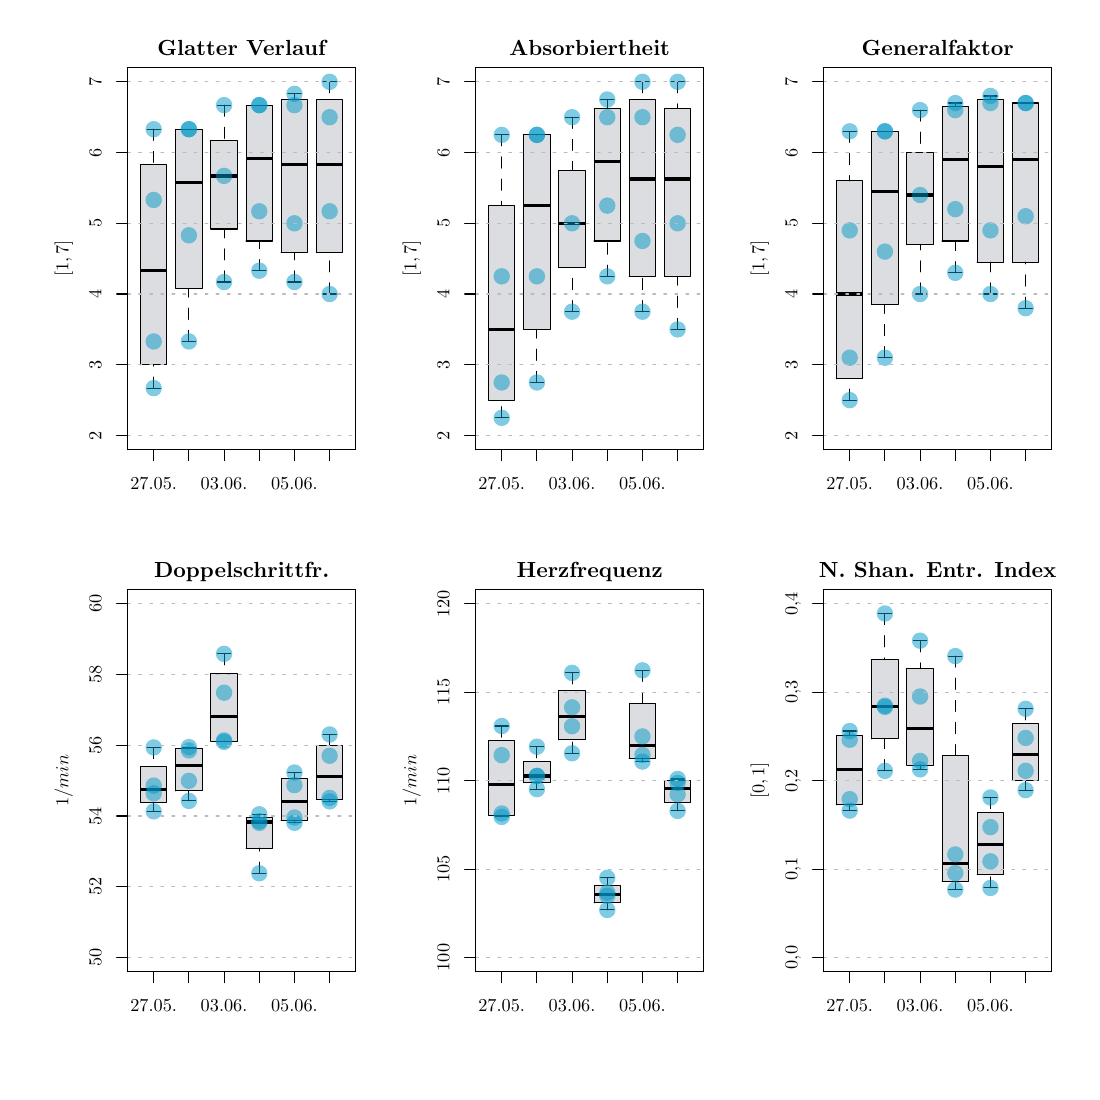
\begin{tikzpicture}[x=1pt,y=1pt]
\definecolor{fillColor}{RGB}{255,255,255}
\path[use as bounding box,fill=fillColor,fill opacity=0.00] (0,0) rectangle (377.25,377.25);
\begin{scope}
\path[clip] ( 36.13,224.76) rectangle (118.52,362.80);
\definecolor{fillColor}{RGB}{186,187,194}

\path[fill=fillColor,fill opacity=0.50] ( 40.78,255.43) --
	( 50.31,255.43) --
	( 50.31,327.78) --
	( 40.78,327.78) --
	cycle;
\definecolor{drawColor}{RGB}{0,0,0}

\path[draw=drawColor,line width= 1.2pt,line join=round] ( 40.78,289.43) -- ( 50.31,289.43);

\path[draw=drawColor,line width= 0.4pt,dash pattern=on 4pt off 4pt ,line join=round,line cap=round] ( 45.54,247.00) -- ( 45.54,255.43);

\path[draw=drawColor,line width= 0.4pt,dash pattern=on 4pt off 4pt ,line join=round,line cap=round] ( 45.54,340.56) -- ( 45.54,327.78);

\path[draw=drawColor,line width= 0.4pt,line join=round,line cap=round] ( 43.16,247.00) -- ( 47.93,247.00);

\path[draw=drawColor,line width= 0.4pt,line join=round,line cap=round] ( 43.16,340.56) -- ( 47.93,340.56);

\path[draw=drawColor,line width= 0.4pt,line join=round,line cap=round] ( 40.78,255.43) --
	( 50.31,255.43) --
	( 50.31,327.78) --
	( 40.78,327.78) --
	( 40.78,255.43);

\path[fill=fillColor,fill opacity=0.50] ( 53.49,283.04) --
	( 63.03,283.04) --
	( 63.03,340.56) --
	( 53.49,340.56) --
	cycle;

\path[draw=drawColor,line width= 1.2pt,line join=round] ( 53.49,321.38) -- ( 63.03,321.38);

\path[draw=drawColor,line width= 0.4pt,dash pattern=on 4pt off 4pt ,line join=round,line cap=round] ( 58.26,263.87) -- ( 58.26,283.04);

\path[draw=drawColor,line width= 0.4pt,dash pattern=on 4pt off 4pt ,line join=round,line cap=round] ( 58.26,340.56) -- ( 58.26,340.56);

\path[draw=drawColor,line width= 0.4pt,line join=round,line cap=round] ( 55.87,263.87) -- ( 60.64,263.87);

\path[draw=drawColor,line width= 0.4pt,line join=round,line cap=round] ( 55.87,340.56) -- ( 60.64,340.56);

\path[draw=drawColor,line width= 0.4pt,line join=round,line cap=round] ( 53.49,283.04) --
	( 63.03,283.04) --
	( 63.03,340.56) --
	( 53.49,340.56) --
	( 53.49,283.04);

\path[fill=fillColor,fill opacity=0.50] ( 66.20,304.51) --
	( 75.74,304.51) --
	( 75.74,336.47) --
	( 66.20,336.47) --
	cycle;

\path[draw=drawColor,line width= 1.2pt,line join=round] ( 66.20,323.69) -- ( 75.74,323.69);

\path[draw=drawColor,line width= 0.4pt,dash pattern=on 4pt off 4pt ,line join=round,line cap=round] ( 70.97,285.34) -- ( 70.97,304.51);

\path[draw=drawColor,line width= 0.4pt,dash pattern=on 4pt off 4pt ,line join=round,line cap=round] ( 70.97,349.25) -- ( 70.97,336.47);

\path[draw=drawColor,line width= 0.4pt,line join=round,line cap=round] ( 68.59,285.34) -- ( 73.36,285.34);

\path[draw=drawColor,line width= 0.4pt,line join=round,line cap=round] ( 68.59,349.25) -- ( 73.36,349.25);

\path[draw=drawColor,line width= 0.4pt,line join=round,line cap=round] ( 66.20,304.51) --
	( 75.74,304.51) --
	( 75.74,336.47) --
	( 66.20,336.47) --
	( 66.20,304.51);

\path[fill=fillColor,fill opacity=0.50] ( 78.92,300.17) --
	( 88.45,300.17) --
	( 88.45,349.25) --
	( 78.92,349.25) --
	cycle;

\path[draw=drawColor,line width= 1.2pt,line join=round] ( 78.92,330.08) -- ( 88.45,330.08);

\path[draw=drawColor,line width= 0.4pt,dash pattern=on 4pt off 4pt ,line join=round,line cap=round] ( 83.69,289.43) -- ( 83.69,300.17);

\path[draw=drawColor,line width= 0.4pt,dash pattern=on 4pt off 4pt ,line join=round,line cap=round] ( 83.69,349.25) -- ( 83.69,349.25);

\path[draw=drawColor,line width= 0.4pt,line join=round,line cap=round] ( 81.30,289.43) -- ( 86.07,289.43);

\path[draw=drawColor,line width= 0.4pt,line join=round,line cap=round] ( 81.30,349.25) -- ( 86.07,349.25);

\path[draw=drawColor,line width= 0.4pt,line join=round,line cap=round] ( 78.92,300.17) --
	( 88.45,300.17) --
	( 88.45,349.25) --
	( 78.92,349.25) --
	( 78.92,300.17);

\path[fill=fillColor,fill opacity=0.50] ( 91.63,295.95) --
	(101.17,295.95) --
	(101.17,351.29) --
	( 91.63,351.29) --
	cycle;

\path[draw=drawColor,line width= 1.2pt,line join=round] ( 91.63,327.90) -- (101.17,327.90);

\path[draw=drawColor,line width= 0.4pt,dash pattern=on 4pt off 4pt ,line join=round,line cap=round] ( 96.40,285.34) -- ( 96.40,295.95);

\path[draw=drawColor,line width= 0.4pt,dash pattern=on 4pt off 4pt ,line join=round,line cap=round] ( 96.40,353.34) -- ( 96.40,351.29);

\path[draw=drawColor,line width= 0.4pt,line join=round,line cap=round] ( 94.02,285.34) -- ( 98.78,285.34);

\path[draw=drawColor,line width= 0.4pt,line join=round,line cap=round] ( 94.02,353.34) -- ( 98.78,353.34);

\path[draw=drawColor,line width= 0.4pt,line join=round,line cap=round] ( 91.63,295.95) --
	(101.17,295.95) --
	(101.17,351.29) --
	( 91.63,351.29) --
	( 91.63,295.95);

\path[fill=fillColor,fill opacity=0.50] (104.35,295.95) --
	(113.88,295.95) --
	(113.88,351.29) --
	(104.35,351.29) --
	cycle;

\path[draw=drawColor,line width= 1.2pt,line join=round] (104.35,327.90) -- (113.88,327.90);

\path[draw=drawColor,line width= 0.4pt,dash pattern=on 4pt off 4pt ,line join=round,line cap=round] (109.11,281.00) -- (109.11,295.95);

\path[draw=drawColor,line width= 0.4pt,dash pattern=on 4pt off 4pt ,line join=round,line cap=round] (109.11,357.68) -- (109.11,351.29);

\path[draw=drawColor,line width= 0.4pt,line join=round,line cap=round] (106.73,281.00) -- (111.50,281.00);

\path[draw=drawColor,line width= 0.4pt,line join=round,line cap=round] (106.73,357.68) -- (111.50,357.68);

\path[draw=drawColor,line width= 0.4pt,line join=round,line cap=round] (104.35,295.95) --
	(113.88,295.95) --
	(113.88,351.29) --
	(104.35,351.29) --
	(104.35,295.95);
\end{scope}
\begin{scope}
\path[clip] (  0.00,  0.00) rectangle (377.25,377.25);
\definecolor{drawColor}{RGB}{0,0,0}

\path[draw=drawColor,line width= 0.4pt,line join=round,line cap=round] ( 45.54,224.76) -- (109.11,224.76);

\path[draw=drawColor,line width= 0.4pt,line join=round,line cap=round] ( 45.54,224.76) -- ( 45.54,220.80);

\path[draw=drawColor,line width= 0.4pt,line join=round,line cap=round] ( 58.26,224.76) -- ( 58.26,220.80);

\path[draw=drawColor,line width= 0.4pt,line join=round,line cap=round] ( 70.97,224.76) -- ( 70.97,220.80);

\path[draw=drawColor,line width= 0.4pt,line join=round,line cap=round] ( 83.69,224.76) -- ( 83.69,220.80);

\path[draw=drawColor,line width= 0.4pt,line join=round,line cap=round] ( 96.40,224.76) -- ( 96.40,220.80);

\path[draw=drawColor,line width= 0.4pt,line join=round,line cap=round] (109.11,224.76) -- (109.11,220.80);

\node[text=drawColor,anchor=base,inner sep=0pt, outer sep=0pt, scale=  0.66] at ( 45.54,210.50) {27.05.};

\node[text=drawColor,anchor=base,inner sep=0pt, outer sep=0pt, scale=  0.66] at ( 70.97,210.50) {03.06.};

\node[text=drawColor,anchor=base,inner sep=0pt, outer sep=0pt, scale=  0.66] at ( 96.40,210.50) {05.06.};

\path[draw=drawColor,line width= 0.4pt,line join=round,line cap=round] ( 36.13,229.87) -- ( 36.13,357.68);

\path[draw=drawColor,line width= 0.4pt,line join=round,line cap=round] ( 36.13,229.87) -- ( 32.17,229.87);

\path[draw=drawColor,line width= 0.4pt,line join=round,line cap=round] ( 36.13,255.43) -- ( 32.17,255.43);

\path[draw=drawColor,line width= 0.4pt,line join=round,line cap=round] ( 36.13,281.00) -- ( 32.17,281.00);

\path[draw=drawColor,line width= 0.4pt,line join=round,line cap=round] ( 36.13,306.56) -- ( 32.17,306.56);

\path[draw=drawColor,line width= 0.4pt,line join=round,line cap=round] ( 36.13,332.12) -- ( 32.17,332.12);

\path[draw=drawColor,line width= 0.4pt,line join=round,line cap=round] ( 36.13,357.68) -- ( 32.17,357.68);

\node[text=drawColor,rotate= 90.00,anchor=base,inner sep=0pt, outer sep=0pt, scale=  0.66] at ( 26.63,229.87) {2};

\node[text=drawColor,rotate= 90.00,anchor=base,inner sep=0pt, outer sep=0pt, scale=  0.66] at ( 26.63,255.43) {3};

\node[text=drawColor,rotate= 90.00,anchor=base,inner sep=0pt, outer sep=0pt, scale=  0.66] at ( 26.63,281.00) {4};

\node[text=drawColor,rotate= 90.00,anchor=base,inner sep=0pt, outer sep=0pt, scale=  0.66] at ( 26.63,306.56) {5};

\node[text=drawColor,rotate= 90.00,anchor=base,inner sep=0pt, outer sep=0pt, scale=  0.66] at ( 26.63,332.12) {6};

\node[text=drawColor,rotate= 90.00,anchor=base,inner sep=0pt, outer sep=0pt, scale=  0.66] at ( 26.63,357.68) {7};
\end{scope}
\begin{scope}
\path[clip] (  0.00,188.62) rectangle (125.75,377.25);
\definecolor{drawColor}{RGB}{0,0,0}

\node[text=drawColor,anchor=base,inner sep=0pt, outer sep=0pt, scale=  0.79] at ( 77.33,367.29) {\bfseries Glatter Verlauf};

\node[text=drawColor,rotate= 90.00,anchor=base,inner sep=0pt, outer sep=0pt, scale=  0.66] at ( 14.75,293.78) {$[1, 7]$};
\end{scope}
\begin{scope}
\path[clip] (  0.00,  0.00) rectangle (377.25,377.25);
\definecolor{drawColor}{RGB}{0,0,0}

\path[draw=drawColor,line width= 0.4pt,line join=round,line cap=round] ( 36.13,224.76) --
	(118.52,224.76) --
	(118.52,362.80) --
	( 36.13,362.80) --
	( 36.13,224.76);
\end{scope}
\begin{scope}
\path[clip] ( 36.13,224.76) rectangle (118.52,362.80);
\definecolor{fillColor}{RGB}{0,152,199}

\path[fill=fillColor,fill opacity=0.50] ( 45.54,247.00) circle (  2.97);

\path[fill=fillColor,fill opacity=0.50] ( 45.54,263.87) circle (  2.97);

\path[fill=fillColor,fill opacity=0.50] ( 45.54,314.99) circle (  2.97);

\path[fill=fillColor,fill opacity=0.50] ( 45.54,340.56) circle (  2.97);

\path[fill=fillColor,fill opacity=0.50] ( 58.26,263.87) circle (  2.97);

\path[fill=fillColor,fill opacity=0.50] ( 58.26,302.21) circle (  2.97);

\path[fill=fillColor,fill opacity=0.50] ( 58.26,340.56) circle (  2.97);

\path[fill=fillColor,fill opacity=0.50] ( 58.26,340.56) circle (  2.97);

\path[fill=fillColor,fill opacity=0.50] ( 70.97,285.34) circle (  2.97);

\path[fill=fillColor,fill opacity=0.50] ( 70.97,323.69) circle (  2.97);

\path[fill=fillColor,fill opacity=0.50] ( 70.97,349.25) circle (  2.97);

\path[fill=fillColor,fill opacity=0.50] ( 83.69,289.43) circle (  2.97);

\path[fill=fillColor,fill opacity=0.50] ( 83.69,310.90) circle (  2.97);

\path[fill=fillColor,fill opacity=0.50] ( 83.69,349.25) circle (  2.97);

\path[fill=fillColor,fill opacity=0.50] ( 83.69,349.25) circle (  2.97);

\path[fill=fillColor,fill opacity=0.50] ( 96.40,285.34) circle (  2.97);

\path[fill=fillColor,fill opacity=0.50] ( 96.40,306.56) circle (  2.97);

\path[fill=fillColor,fill opacity=0.50] ( 96.40,353.34) circle (  2.97);

\path[fill=fillColor,fill opacity=0.50] ( 96.40,349.25) circle (  2.97);

\path[fill=fillColor,fill opacity=0.50] (109.11,281.00) circle (  2.97);

\path[fill=fillColor,fill opacity=0.50] (109.11,310.90) circle (  2.97);

\path[fill=fillColor,fill opacity=0.50] (109.11,344.90) circle (  2.97);

\path[fill=fillColor,fill opacity=0.50] (109.11,357.68) circle (  2.97);
\definecolor{drawColor}{RGB}{186,187,194}

\path[draw=drawColor,line width= 0.4pt,dash pattern=on 1pt off 3pt ,line join=round,line cap=round] ( 36.13,229.87) -- (118.52,229.87);

\path[draw=drawColor,line width= 0.4pt,dash pattern=on 1pt off 3pt ,line join=round,line cap=round] ( 36.13,255.43) -- (118.52,255.43);

\path[draw=drawColor,line width= 0.4pt,dash pattern=on 1pt off 3pt ,line join=round,line cap=round] ( 36.13,281.00) -- (118.52,281.00);

\path[draw=drawColor,line width= 0.4pt,dash pattern=on 1pt off 3pt ,line join=round,line cap=round] ( 36.13,306.56) -- (118.52,306.56);

\path[draw=drawColor,line width= 0.4pt,dash pattern=on 1pt off 3pt ,line join=round,line cap=round] ( 36.13,332.12) -- (118.52,332.12);

\path[draw=drawColor,line width= 0.4pt,dash pattern=on 1pt off 3pt ,line join=round,line cap=round] ( 36.13,357.68) -- (118.52,357.68);
\end{scope}
\begin{scope}
\path[clip] (  0.00,  0.00) rectangle (377.25,377.25);
\definecolor{drawColor}{RGB}{0,0,0}

\path[draw=drawColor,line width= 0.4pt,line join=round,line cap=round] ( 36.13,224.76) --
	(118.52,224.76) --
	(118.52,362.80) --
	( 36.13,362.80) --
	( 36.13,224.76);
\end{scope}
\begin{scope}
\path[clip] (161.88,224.76) rectangle (244.27,362.80);
\definecolor{fillColor}{RGB}{186,187,194}

\path[fill=fillColor,fill opacity=0.50] (166.53,242.65) --
	(176.06,242.65) --
	(176.06,312.95) --
	(166.53,312.95) --
	cycle;
\definecolor{drawColor}{RGB}{0,0,0}

\path[draw=drawColor,line width= 1.2pt,line join=round] (166.53,268.22) -- (176.06,268.22);

\path[draw=drawColor,line width= 0.4pt,dash pattern=on 4pt off 4pt ,line join=round,line cap=round] (171.29,236.26) -- (171.29,242.65);

\path[draw=drawColor,line width= 0.4pt,dash pattern=on 4pt off 4pt ,line join=round,line cap=round] (171.29,338.51) -- (171.29,312.95);

\path[draw=drawColor,line width= 0.4pt,line join=round,line cap=round] (168.91,236.26) -- (173.68,236.26);

\path[draw=drawColor,line width= 0.4pt,line join=round,line cap=round] (168.91,338.51) -- (173.68,338.51);

\path[draw=drawColor,line width= 0.4pt,line join=round,line cap=round] (166.53,242.65) --
	(176.06,242.65) --
	(176.06,312.95) --
	(166.53,312.95) --
	(166.53,242.65);

\path[fill=fillColor,fill opacity=0.50] (179.24,268.22) --
	(188.78,268.22) --
	(188.78,338.51) --
	(179.24,338.51) --
	cycle;

\path[draw=drawColor,line width= 1.2pt,line join=round] (179.24,312.95) -- (188.78,312.95);

\path[draw=drawColor,line width= 0.4pt,dash pattern=on 4pt off 4pt ,line join=round,line cap=round] (184.01,249.04) -- (184.01,268.22);

\path[draw=drawColor,line width= 0.4pt,dash pattern=on 4pt off 4pt ,line join=round,line cap=round] (184.01,338.51) -- (184.01,338.51);

\path[draw=drawColor,line width= 0.4pt,line join=round,line cap=round] (181.62,249.04) -- (186.39,249.04);

\path[draw=drawColor,line width= 0.4pt,line join=round,line cap=round] (181.62,338.51) -- (186.39,338.51);

\path[draw=drawColor,line width= 0.4pt,line join=round,line cap=round] (179.24,268.22) --
	(188.78,268.22) --
	(188.78,338.51) --
	(179.24,338.51) --
	(179.24,268.22);

\path[fill=fillColor,fill opacity=0.50] (191.95,290.58) --
	(201.49,290.58) --
	(201.49,325.73) --
	(191.95,325.73) --
	cycle;

\path[draw=drawColor,line width= 1.2pt,line join=round] (191.95,306.56) -- (201.49,306.56);

\path[draw=drawColor,line width= 0.4pt,dash pattern=on 4pt off 4pt ,line join=round,line cap=round] (196.72,274.61) -- (196.72,290.58);

\path[draw=drawColor,line width= 0.4pt,dash pattern=on 4pt off 4pt ,line join=round,line cap=round] (196.72,344.90) -- (196.72,325.73);

\path[draw=drawColor,line width= 0.4pt,line join=round,line cap=round] (194.34,274.61) -- (199.11,274.61);

\path[draw=drawColor,line width= 0.4pt,line join=round,line cap=round] (194.34,344.90) -- (199.11,344.90);

\path[draw=drawColor,line width= 0.4pt,line join=round,line cap=round] (191.95,290.58) --
	(201.49,290.58) --
	(201.49,325.73) --
	(191.95,325.73) --
	(191.95,290.58);

\path[fill=fillColor,fill opacity=0.50] (204.67,300.17) --
	(214.20,300.17) --
	(214.20,348.10) --
	(204.67,348.10) --
	cycle;

\path[draw=drawColor,line width= 1.2pt,line join=round] (204.67,328.93) -- (214.20,328.93);

\path[draw=drawColor,line width= 0.4pt,dash pattern=on 4pt off 4pt ,line join=round,line cap=round] (209.44,287.39) -- (209.44,300.17);

\path[draw=drawColor,line width= 0.4pt,dash pattern=on 4pt off 4pt ,line join=round,line cap=round] (209.44,351.29) -- (209.44,348.10);

\path[draw=drawColor,line width= 0.4pt,line join=round,line cap=round] (207.05,287.39) -- (211.82,287.39);

\path[draw=drawColor,line width= 0.4pt,line join=round,line cap=round] (207.05,351.29) -- (211.82,351.29);

\path[draw=drawColor,line width= 0.4pt,line join=round,line cap=round] (204.67,300.17) --
	(214.20,300.17) --
	(214.20,348.10) --
	(204.67,348.10) --
	(204.67,300.17);

\path[fill=fillColor,fill opacity=0.50] (217.38,287.39) --
	(226.92,287.39) --
	(226.92,351.29) --
	(217.38,351.29) --
	cycle;

\path[draw=drawColor,line width= 1.2pt,line join=round] (217.38,322.53) -- (226.92,322.53);

\path[draw=drawColor,line width= 0.4pt,dash pattern=on 4pt off 4pt ,line join=round,line cap=round] (222.15,274.61) -- (222.15,287.39);

\path[draw=drawColor,line width= 0.4pt,dash pattern=on 4pt off 4pt ,line join=round,line cap=round] (222.15,357.68) -- (222.15,351.29);

\path[draw=drawColor,line width= 0.4pt,line join=round,line cap=round] (219.77,274.61) -- (224.53,274.61);

\path[draw=drawColor,line width= 0.4pt,line join=round,line cap=round] (219.77,357.68) -- (224.53,357.68);

\path[draw=drawColor,line width= 0.4pt,line join=round,line cap=round] (217.38,287.39) --
	(226.92,287.39) --
	(226.92,351.29) --
	(217.38,351.29) --
	(217.38,287.39);

\path[fill=fillColor,fill opacity=0.50] (230.10,287.39) --
	(239.63,287.39) --
	(239.63,348.10) --
	(230.10,348.10) --
	cycle;

\path[draw=drawColor,line width= 1.2pt,line join=round] (230.10,322.53) -- (239.63,322.53);

\path[draw=drawColor,line width= 0.4pt,dash pattern=on 4pt off 4pt ,line join=round,line cap=round] (234.86,268.22) -- (234.86,287.39);

\path[draw=drawColor,line width= 0.4pt,dash pattern=on 4pt off 4pt ,line join=round,line cap=round] (234.86,357.68) -- (234.86,348.10);

\path[draw=drawColor,line width= 0.4pt,line join=round,line cap=round] (232.48,268.22) -- (237.25,268.22);

\path[draw=drawColor,line width= 0.4pt,line join=round,line cap=round] (232.48,357.68) -- (237.25,357.68);

\path[draw=drawColor,line width= 0.4pt,line join=round,line cap=round] (230.10,287.39) --
	(239.63,287.39) --
	(239.63,348.10) --
	(230.10,348.10) --
	(230.10,287.39);
\end{scope}
\begin{scope}
\path[clip] (  0.00,  0.00) rectangle (377.25,377.25);
\definecolor{drawColor}{RGB}{0,0,0}

\path[draw=drawColor,line width= 0.4pt,line join=round,line cap=round] (171.29,224.76) -- (234.86,224.76);

\path[draw=drawColor,line width= 0.4pt,line join=round,line cap=round] (171.29,224.76) -- (171.29,220.80);

\path[draw=drawColor,line width= 0.4pt,line join=round,line cap=round] (184.01,224.76) -- (184.01,220.80);

\path[draw=drawColor,line width= 0.4pt,line join=round,line cap=round] (196.72,224.76) -- (196.72,220.80);

\path[draw=drawColor,line width= 0.4pt,line join=round,line cap=round] (209.44,224.76) -- (209.44,220.80);

\path[draw=drawColor,line width= 0.4pt,line join=round,line cap=round] (222.15,224.76) -- (222.15,220.80);

\path[draw=drawColor,line width= 0.4pt,line join=round,line cap=round] (234.86,224.76) -- (234.86,220.80);

\node[text=drawColor,anchor=base,inner sep=0pt, outer sep=0pt, scale=  0.66] at (171.29,210.50) {27.05.};

\node[text=drawColor,anchor=base,inner sep=0pt, outer sep=0pt, scale=  0.66] at (196.72,210.50) {03.06.};

\node[text=drawColor,anchor=base,inner sep=0pt, outer sep=0pt, scale=  0.66] at (222.15,210.50) {05.06.};

\path[draw=drawColor,line width= 0.4pt,line join=round,line cap=round] (161.88,229.87) -- (161.88,357.68);

\path[draw=drawColor,line width= 0.4pt,line join=round,line cap=round] (161.88,229.87) -- (157.92,229.87);

\path[draw=drawColor,line width= 0.4pt,line join=round,line cap=round] (161.88,255.43) -- (157.92,255.43);

\path[draw=drawColor,line width= 0.4pt,line join=round,line cap=round] (161.88,281.00) -- (157.92,281.00);

\path[draw=drawColor,line width= 0.4pt,line join=round,line cap=round] (161.88,306.56) -- (157.92,306.56);

\path[draw=drawColor,line width= 0.4pt,line join=round,line cap=round] (161.88,332.12) -- (157.92,332.12);

\path[draw=drawColor,line width= 0.4pt,line join=round,line cap=round] (161.88,357.68) -- (157.92,357.68);

\node[text=drawColor,rotate= 90.00,anchor=base,inner sep=0pt, outer sep=0pt, scale=  0.66] at (152.38,229.87) {2};

\node[text=drawColor,rotate= 90.00,anchor=base,inner sep=0pt, outer sep=0pt, scale=  0.66] at (152.38,255.43) {3};

\node[text=drawColor,rotate= 90.00,anchor=base,inner sep=0pt, outer sep=0pt, scale=  0.66] at (152.38,281.00) {4};

\node[text=drawColor,rotate= 90.00,anchor=base,inner sep=0pt, outer sep=0pt, scale=  0.66] at (152.38,306.56) {5};

\node[text=drawColor,rotate= 90.00,anchor=base,inner sep=0pt, outer sep=0pt, scale=  0.66] at (152.38,332.12) {6};

\node[text=drawColor,rotate= 90.00,anchor=base,inner sep=0pt, outer sep=0pt, scale=  0.66] at (152.38,357.68) {7};
\end{scope}
\begin{scope}
\path[clip] (125.75,188.62) rectangle (251.50,377.25);
\definecolor{drawColor}{RGB}{0,0,0}

\node[text=drawColor,anchor=base,inner sep=0pt, outer sep=0pt, scale=  0.79] at (203.08,367.29) {\bfseries Absorbiertheit};

\node[text=drawColor,rotate= 90.00,anchor=base,inner sep=0pt, outer sep=0pt, scale=  0.66] at (140.50,293.78) {$[1, 7]$};
\end{scope}
\begin{scope}
\path[clip] (  0.00,  0.00) rectangle (377.25,377.25);
\definecolor{drawColor}{RGB}{0,0,0}

\path[draw=drawColor,line width= 0.4pt,line join=round,line cap=round] (161.88,224.76) --
	(244.27,224.76) --
	(244.27,362.80) --
	(161.88,362.80) --
	(161.88,224.76);
\end{scope}
\begin{scope}
\path[clip] (161.88,224.76) rectangle (244.27,362.80);
\definecolor{fillColor}{RGB}{0,152,199}

\path[fill=fillColor,fill opacity=0.50] (171.29,236.26) circle (  2.97);

\path[fill=fillColor,fill opacity=0.50] (171.29,249.04) circle (  2.97);

\path[fill=fillColor,fill opacity=0.50] (171.29,287.39) circle (  2.97);

\path[fill=fillColor,fill opacity=0.50] (171.29,338.51) circle (  2.97);

\path[fill=fillColor,fill opacity=0.50] (184.01,249.04) circle (  2.97);

\path[fill=fillColor,fill opacity=0.50] (184.01,287.39) circle (  2.97);

\path[fill=fillColor,fill opacity=0.50] (184.01,338.51) circle (  2.97);

\path[fill=fillColor,fill opacity=0.50] (184.01,338.51) circle (  2.97);

\path[fill=fillColor,fill opacity=0.50] (196.72,274.61) circle (  2.97);

\path[fill=fillColor,fill opacity=0.50] (196.72,306.56) circle (  2.97);

\path[fill=fillColor,fill opacity=0.50] (196.72,344.90) circle (  2.97);

\path[fill=fillColor,fill opacity=0.50] (209.44,287.39) circle (  2.97);

\path[fill=fillColor,fill opacity=0.50] (209.44,312.95) circle (  2.97);

\path[fill=fillColor,fill opacity=0.50] (209.44,344.90) circle (  2.97);

\path[fill=fillColor,fill opacity=0.50] (209.44,351.29) circle (  2.97);

\path[fill=fillColor,fill opacity=0.50] (222.15,274.61) circle (  2.97);

\path[fill=fillColor,fill opacity=0.50] (222.15,300.17) circle (  2.97);

\path[fill=fillColor,fill opacity=0.50] (222.15,344.90) circle (  2.97);

\path[fill=fillColor,fill opacity=0.50] (222.15,357.68) circle (  2.97);

\path[fill=fillColor,fill opacity=0.50] (234.86,268.22) circle (  2.97);

\path[fill=fillColor,fill opacity=0.50] (234.86,306.56) circle (  2.97);

\path[fill=fillColor,fill opacity=0.50] (234.86,357.68) circle (  2.97);

\path[fill=fillColor,fill opacity=0.50] (234.86,338.51) circle (  2.97);
\definecolor{drawColor}{RGB}{186,187,194}

\path[draw=drawColor,line width= 0.4pt,dash pattern=on 1pt off 3pt ,line join=round,line cap=round] (161.88,229.87) -- (244.27,229.87);

\path[draw=drawColor,line width= 0.4pt,dash pattern=on 1pt off 3pt ,line join=round,line cap=round] (161.88,255.43) -- (244.27,255.43);

\path[draw=drawColor,line width= 0.4pt,dash pattern=on 1pt off 3pt ,line join=round,line cap=round] (161.88,281.00) -- (244.27,281.00);

\path[draw=drawColor,line width= 0.4pt,dash pattern=on 1pt off 3pt ,line join=round,line cap=round] (161.88,306.56) -- (244.27,306.56);

\path[draw=drawColor,line width= 0.4pt,dash pattern=on 1pt off 3pt ,line join=round,line cap=round] (161.88,332.12) -- (244.27,332.12);

\path[draw=drawColor,line width= 0.4pt,dash pattern=on 1pt off 3pt ,line join=round,line cap=round] (161.88,357.68) -- (244.27,357.68);
\end{scope}
\begin{scope}
\path[clip] (  0.00,  0.00) rectangle (377.25,377.25);
\definecolor{drawColor}{RGB}{0,0,0}

\path[draw=drawColor,line width= 0.4pt,line join=round,line cap=round] (161.88,224.76) --
	(244.27,224.76) --
	(244.27,362.80) --
	(161.88,362.80) --
	(161.88,224.76);
\end{scope}
\begin{scope}
\path[clip] (287.63,224.76) rectangle (370.02,362.80);
\definecolor{fillColor}{RGB}{186,187,194}

\path[fill=fillColor,fill opacity=0.50] (292.28,250.32) --
	(301.81,250.32) --
	(301.81,321.90) --
	(292.28,321.90) --
	cycle;
\definecolor{drawColor}{RGB}{0,0,0}

\path[draw=drawColor,line width= 1.2pt,line join=round] (292.28,281.00) -- (301.81,281.00);

\path[draw=drawColor,line width= 0.4pt,dash pattern=on 4pt off 4pt ,line join=round,line cap=round] (297.04,242.65) -- (297.04,250.32);

\path[draw=drawColor,line width= 0.4pt,dash pattern=on 4pt off 4pt ,line join=round,line cap=round] (297.04,339.79) -- (297.04,321.90);

\path[draw=drawColor,line width= 0.4pt,line join=round,line cap=round] (294.66,242.65) -- (299.43,242.65);

\path[draw=drawColor,line width= 0.4pt,line join=round,line cap=round] (294.66,339.79) -- (299.43,339.79);

\path[draw=drawColor,line width= 0.4pt,line join=round,line cap=round] (292.28,250.32) --
	(301.81,250.32) --
	(301.81,321.90) --
	(292.28,321.90) --
	(292.28,250.32);

\path[fill=fillColor,fill opacity=0.50] (304.99,277.16) --
	(314.53,277.16) --
	(314.53,339.79) --
	(304.99,339.79) --
	cycle;

\path[draw=drawColor,line width= 1.2pt,line join=round] (304.99,318.06) -- (314.53,318.06);

\path[draw=drawColor,line width= 0.4pt,dash pattern=on 4pt off 4pt ,line join=round,line cap=round] (309.76,257.99) -- (309.76,277.16);

\path[draw=drawColor,line width= 0.4pt,dash pattern=on 4pt off 4pt ,line join=round,line cap=round] (309.76,339.79) -- (309.76,339.79);

\path[draw=drawColor,line width= 0.4pt,line join=round,line cap=round] (307.37,257.99) -- (312.14,257.99);

\path[draw=drawColor,line width= 0.4pt,line join=round,line cap=round] (307.37,339.79) -- (312.14,339.79);

\path[draw=drawColor,line width= 0.4pt,line join=round,line cap=round] (304.99,277.16) --
	(314.53,277.16) --
	(314.53,339.79) --
	(304.99,339.79) --
	(304.99,277.16);

\path[fill=fillColor,fill opacity=0.50] (317.70,298.89) --
	(327.24,298.89) --
	(327.24,332.12) --
	(317.70,332.12) --
	cycle;

\path[draw=drawColor,line width= 1.2pt,line join=round] (317.70,316.78) -- (327.24,316.78);

\path[draw=drawColor,line width= 0.4pt,dash pattern=on 4pt off 4pt ,line join=round,line cap=round] (322.47,281.00) -- (322.47,298.89);

\path[draw=drawColor,line width= 0.4pt,dash pattern=on 4pt off 4pt ,line join=round,line cap=round] (322.47,347.46) -- (322.47,332.12);

\path[draw=drawColor,line width= 0.4pt,line join=round,line cap=round] (320.09,281.00) -- (324.86,281.00);

\path[draw=drawColor,line width= 0.4pt,line join=round,line cap=round] (320.09,347.46) -- (324.86,347.46);

\path[draw=drawColor,line width= 0.4pt,line join=round,line cap=round] (317.70,298.89) --
	(327.24,298.89) --
	(327.24,332.12) --
	(317.70,332.12) --
	(317.70,298.89);

\path[fill=fillColor,fill opacity=0.50] (330.42,300.17) --
	(339.95,300.17) --
	(339.95,348.74) --
	(330.42,348.74) --
	cycle;

\path[draw=drawColor,line width= 1.2pt,line join=round] (330.42,329.56) -- (339.95,329.56);

\path[draw=drawColor,line width= 0.4pt,dash pattern=on 4pt off 4pt ,line join=round,line cap=round] (335.19,288.67) -- (335.19,300.17);

\path[draw=drawColor,line width= 0.4pt,dash pattern=on 4pt off 4pt ,line join=round,line cap=round] (335.19,350.01) -- (335.19,348.74);

\path[draw=drawColor,line width= 0.4pt,line join=round,line cap=round] (332.80,288.67) -- (337.57,288.67);

\path[draw=drawColor,line width= 0.4pt,line join=round,line cap=round] (332.80,350.01) -- (337.57,350.01);

\path[draw=drawColor,line width= 0.4pt,line join=round,line cap=round] (330.42,300.17) --
	(339.95,300.17) --
	(339.95,348.74) --
	(330.42,348.74) --
	(330.42,300.17);

\path[fill=fillColor,fill opacity=0.50] (343.13,292.50) --
	(352.67,292.50) --
	(352.67,351.29) --
	(343.13,351.29) --
	cycle;

\path[draw=drawColor,line width= 1.2pt,line join=round] (343.13,327.01) -- (352.67,327.01);

\path[draw=drawColor,line width= 0.4pt,dash pattern=on 4pt off 4pt ,line join=round,line cap=round] (347.90,281.00) -- (347.90,292.50);

\path[draw=drawColor,line width= 0.4pt,dash pattern=on 4pt off 4pt ,line join=round,line cap=round] (347.90,352.57) -- (347.90,351.29);

\path[draw=drawColor,line width= 0.4pt,line join=round,line cap=round] (345.52,281.00) -- (350.28,281.00);

\path[draw=drawColor,line width= 0.4pt,line join=round,line cap=round] (345.52,352.57) -- (350.28,352.57);

\path[draw=drawColor,line width= 0.4pt,line join=round,line cap=round] (343.13,292.50) --
	(352.67,292.50) --
	(352.67,351.29) --
	(343.13,351.29) --
	(343.13,292.50);

\path[fill=fillColor,fill opacity=0.50] (355.85,292.50) --
	(365.38,292.50) --
	(365.38,350.01) --
	(355.85,350.01) --
	cycle;

\path[draw=drawColor,line width= 1.2pt,line join=round] (355.85,329.56) -- (365.38,329.56);

\path[draw=drawColor,line width= 0.4pt,dash pattern=on 4pt off 4pt ,line join=round,line cap=round] (360.61,275.88) -- (360.61,292.50);

\path[draw=drawColor,line width= 0.4pt,dash pattern=on 4pt off 4pt ,line join=round,line cap=round] (360.61,350.01) -- (360.61,350.01);

\path[draw=drawColor,line width= 0.4pt,line join=round,line cap=round] (358.23,275.88) -- (363.00,275.88);

\path[draw=drawColor,line width= 0.4pt,line join=round,line cap=round] (358.23,350.01) -- (363.00,350.01);

\path[draw=drawColor,line width= 0.4pt,line join=round,line cap=round] (355.85,292.50) --
	(365.38,292.50) --
	(365.38,350.01) --
	(355.85,350.01) --
	(355.85,292.50);
\end{scope}
\begin{scope}
\path[clip] (  0.00,  0.00) rectangle (377.25,377.25);
\definecolor{drawColor}{RGB}{0,0,0}

\path[draw=drawColor,line width= 0.4pt,line join=round,line cap=round] (297.04,224.76) -- (360.61,224.76);

\path[draw=drawColor,line width= 0.4pt,line join=round,line cap=round] (297.04,224.76) -- (297.04,220.80);

\path[draw=drawColor,line width= 0.4pt,line join=round,line cap=round] (309.76,224.76) -- (309.76,220.80);

\path[draw=drawColor,line width= 0.4pt,line join=round,line cap=round] (322.47,224.76) -- (322.47,220.80);

\path[draw=drawColor,line width= 0.4pt,line join=round,line cap=round] (335.19,224.76) -- (335.19,220.80);

\path[draw=drawColor,line width= 0.4pt,line join=round,line cap=round] (347.90,224.76) -- (347.90,220.80);

\path[draw=drawColor,line width= 0.4pt,line join=round,line cap=round] (360.61,224.76) -- (360.61,220.80);

\node[text=drawColor,anchor=base,inner sep=0pt, outer sep=0pt, scale=  0.66] at (297.04,210.50) {27.05.};

\node[text=drawColor,anchor=base,inner sep=0pt, outer sep=0pt, scale=  0.66] at (322.47,210.50) {03.06.};

\node[text=drawColor,anchor=base,inner sep=0pt, outer sep=0pt, scale=  0.66] at (347.90,210.50) {05.06.};

\path[draw=drawColor,line width= 0.4pt,line join=round,line cap=round] (287.63,229.87) -- (287.63,357.68);

\path[draw=drawColor,line width= 0.4pt,line join=round,line cap=round] (287.63,229.87) -- (283.67,229.87);

\path[draw=drawColor,line width= 0.4pt,line join=round,line cap=round] (287.63,255.43) -- (283.67,255.43);

\path[draw=drawColor,line width= 0.4pt,line join=round,line cap=round] (287.63,281.00) -- (283.67,281.00);

\path[draw=drawColor,line width= 0.4pt,line join=round,line cap=round] (287.63,306.56) -- (283.67,306.56);

\path[draw=drawColor,line width= 0.4pt,line join=round,line cap=round] (287.63,332.12) -- (283.67,332.12);

\path[draw=drawColor,line width= 0.4pt,line join=round,line cap=round] (287.63,357.68) -- (283.67,357.68);

\node[text=drawColor,rotate= 90.00,anchor=base,inner sep=0pt, outer sep=0pt, scale=  0.66] at (278.13,229.87) {2};

\node[text=drawColor,rotate= 90.00,anchor=base,inner sep=0pt, outer sep=0pt, scale=  0.66] at (278.13,255.43) {3};

\node[text=drawColor,rotate= 90.00,anchor=base,inner sep=0pt, outer sep=0pt, scale=  0.66] at (278.13,281.00) {4};

\node[text=drawColor,rotate= 90.00,anchor=base,inner sep=0pt, outer sep=0pt, scale=  0.66] at (278.13,306.56) {5};

\node[text=drawColor,rotate= 90.00,anchor=base,inner sep=0pt, outer sep=0pt, scale=  0.66] at (278.13,332.12) {6};

\node[text=drawColor,rotate= 90.00,anchor=base,inner sep=0pt, outer sep=0pt, scale=  0.66] at (278.13,357.68) {7};
\end{scope}
\begin{scope}
\path[clip] (251.50,188.62) rectangle (377.25,377.25);
\definecolor{drawColor}{RGB}{0,0,0}

\node[text=drawColor,anchor=base,inner sep=0pt, outer sep=0pt, scale=  0.79] at (328.83,367.29) {\bfseries Generalfaktor};

\node[text=drawColor,rotate= 90.00,anchor=base,inner sep=0pt, outer sep=0pt, scale=  0.66] at (266.25,293.78) {$[1, 7]$};
\end{scope}
\begin{scope}
\path[clip] (  0.00,  0.00) rectangle (377.25,377.25);
\definecolor{drawColor}{RGB}{0,0,0}

\path[draw=drawColor,line width= 0.4pt,line join=round,line cap=round] (287.63,224.76) --
	(370.02,224.76) --
	(370.02,362.80) --
	(287.63,362.80) --
	(287.63,224.76);
\end{scope}
\begin{scope}
\path[clip] (287.63,224.76) rectangle (370.02,362.80);
\definecolor{fillColor}{RGB}{0,152,199}

\path[fill=fillColor,fill opacity=0.50] (297.04,242.65) circle (  2.97);

\path[fill=fillColor,fill opacity=0.50] (297.04,257.99) circle (  2.97);

\path[fill=fillColor,fill opacity=0.50] (297.04,304.00) circle (  2.97);

\path[fill=fillColor,fill opacity=0.50] (297.04,339.79) circle (  2.97);

\path[fill=fillColor,fill opacity=0.50] (309.76,257.99) circle (  2.97);

\path[fill=fillColor,fill opacity=0.50] (309.76,296.33) circle (  2.97);

\path[fill=fillColor,fill opacity=0.50] (309.76,339.79) circle (  2.97);

\path[fill=fillColor,fill opacity=0.50] (309.76,339.79) circle (  2.97);

\path[fill=fillColor,fill opacity=0.50] (322.47,281.00) circle (  2.97);

\path[fill=fillColor,fill opacity=0.50] (322.47,316.78) circle (  2.97);

\path[fill=fillColor,fill opacity=0.50] (322.47,347.46) circle (  2.97);

\path[fill=fillColor,fill opacity=0.50] (335.19,288.67) circle (  2.97);

\path[fill=fillColor,fill opacity=0.50] (335.19,311.67) circle (  2.97);

\path[fill=fillColor,fill opacity=0.50] (335.19,347.46) circle (  2.97);

\path[fill=fillColor,fill opacity=0.50] (335.19,350.01) circle (  2.97);

\path[fill=fillColor,fill opacity=0.50] (347.90,281.00) circle (  2.97);

\path[fill=fillColor,fill opacity=0.50] (347.90,304.00) circle (  2.97);

\path[fill=fillColor,fill opacity=0.50] (347.90,350.01) circle (  2.97);

\path[fill=fillColor,fill opacity=0.50] (347.90,352.57) circle (  2.97);

\path[fill=fillColor,fill opacity=0.50] (360.61,275.88) circle (  2.97);

\path[fill=fillColor,fill opacity=0.50] (360.61,309.11) circle (  2.97);

\path[fill=fillColor,fill opacity=0.50] (360.61,350.01) circle (  2.97);

\path[fill=fillColor,fill opacity=0.50] (360.61,350.01) circle (  2.97);
\definecolor{drawColor}{RGB}{186,187,194}

\path[draw=drawColor,line width= 0.4pt,dash pattern=on 1pt off 3pt ,line join=round,line cap=round] (287.63,229.87) -- (370.02,229.87);

\path[draw=drawColor,line width= 0.4pt,dash pattern=on 1pt off 3pt ,line join=round,line cap=round] (287.63,255.43) -- (370.02,255.43);

\path[draw=drawColor,line width= 0.4pt,dash pattern=on 1pt off 3pt ,line join=round,line cap=round] (287.63,281.00) -- (370.02,281.00);

\path[draw=drawColor,line width= 0.4pt,dash pattern=on 1pt off 3pt ,line join=round,line cap=round] (287.63,306.56) -- (370.02,306.56);

\path[draw=drawColor,line width= 0.4pt,dash pattern=on 1pt off 3pt ,line join=round,line cap=round] (287.63,332.12) -- (370.02,332.12);

\path[draw=drawColor,line width= 0.4pt,dash pattern=on 1pt off 3pt ,line join=round,line cap=round] (287.63,357.68) -- (370.02,357.68);
\end{scope}
\begin{scope}
\path[clip] (  0.00,  0.00) rectangle (377.25,377.25);
\definecolor{drawColor}{RGB}{0,0,0}

\path[draw=drawColor,line width= 0.4pt,line join=round,line cap=round] (287.63,224.76) --
	(370.02,224.76) --
	(370.02,362.80) --
	(287.63,362.80) --
	(287.63,224.76);
\end{scope}
\begin{scope}
\path[clip] ( 36.13, 36.13) rectangle (118.52,174.17);
\definecolor{fillColor}{RGB}{186,187,194}

\path[fill=fillColor,fill opacity=0.50] ( 40.78, 97.32) --
	( 50.31, 97.32) --
	( 50.31,110.27) --
	( 40.78,110.27) --
	cycle;
\definecolor{drawColor}{RGB}{0,0,0}

\path[draw=drawColor,line width= 1.2pt,line join=round] ( 40.78,101.98) -- ( 50.31,101.98);

\path[draw=drawColor,line width= 0.4pt,dash pattern=on 4pt off 4pt ,line join=round,line cap=round] ( 45.54, 94.06) -- ( 45.54, 97.32);

\path[draw=drawColor,line width= 0.4pt,dash pattern=on 4pt off 4pt ,line join=round,line cap=round] ( 45.54,117.17) -- ( 45.54,110.27);

\path[draw=drawColor,line width= 0.4pt,line join=round,line cap=round] ( 43.16, 94.06) -- ( 47.93, 94.06);

\path[draw=drawColor,line width= 0.4pt,line join=round,line cap=round] ( 43.16,117.17) -- ( 47.93,117.17);

\path[draw=drawColor,line width= 0.4pt,line join=round,line cap=round] ( 40.78, 97.32) --
	( 50.31, 97.32) --
	( 50.31,110.27) --
	( 40.78,110.27) --
	( 40.78, 97.32);

\path[fill=fillColor,fill opacity=0.50] ( 53.49,101.46) --
	( 63.03,101.46) --
	( 63.03,116.69) --
	( 53.49,116.69) --
	cycle;

\path[draw=drawColor,line width= 1.2pt,line join=round] ( 53.49,110.59) -- ( 63.03,110.59);

\path[draw=drawColor,line width= 0.4pt,dash pattern=on 4pt off 4pt ,line join=round,line cap=round] ( 58.26, 97.83) -- ( 58.26,101.46);

\path[draw=drawColor,line width= 0.4pt,dash pattern=on 4pt off 4pt ,line join=round,line cap=round] ( 58.26,117.29) -- ( 58.26,116.69);

\path[draw=drawColor,line width= 0.4pt,line join=round,line cap=round] ( 55.87, 97.83) -- ( 60.64, 97.83);

\path[draw=drawColor,line width= 0.4pt,line join=round,line cap=round] ( 55.87,117.29) -- ( 60.64,117.29);

\path[draw=drawColor,line width= 0.4pt,line join=round,line cap=round] ( 53.49,101.46) --
	( 63.03,101.46) --
	( 63.03,116.69) --
	( 53.49,116.69) --
	( 53.49,101.46);

\path[fill=fillColor,fill opacity=0.50] ( 66.20,119.45) --
	( 75.74,119.45) --
	( 75.74,143.96) --
	( 66.20,143.96) --
	cycle;

\path[draw=drawColor,line width= 1.2pt,line join=round] ( 66.20,128.33) -- ( 75.74,128.33);

\path[draw=drawColor,line width= 0.4pt,dash pattern=on 4pt off 4pt ,line join=round,line cap=round] ( 70.97,119.17) -- ( 70.97,119.45);

\path[draw=drawColor,line width= 0.4pt,dash pattern=on 4pt off 4pt ,line join=round,line cap=round] ( 70.97,150.97) -- ( 70.97,143.96);

\path[draw=drawColor,line width= 0.4pt,line join=round,line cap=round] ( 68.59,119.17) -- ( 73.36,119.17);

\path[draw=drawColor,line width= 0.4pt,line join=round,line cap=round] ( 68.59,150.97) -- ( 73.36,150.97);

\path[draw=drawColor,line width= 0.4pt,line join=round,line cap=round] ( 66.20,119.45) --
	( 75.74,119.45) --
	( 75.74,143.96) --
	( 66.20,143.96) --
	( 66.20,119.45);

\path[fill=fillColor,fill opacity=0.50] ( 78.92, 80.79) --
	( 88.45, 80.79) --
	( 88.45, 91.76) --
	( 78.92, 91.76) --
	cycle;

\path[draw=drawColor,line width= 1.2pt,line join=round] ( 78.92, 90.20) -- ( 88.45, 90.20);

\path[draw=drawColor,line width= 0.4pt,dash pattern=on 4pt off 4pt ,line join=round,line cap=round] ( 83.69, 71.69) -- ( 83.69, 80.79);

\path[draw=drawColor,line width= 0.4pt,dash pattern=on 4pt off 4pt ,line join=round,line cap=round] ( 83.69, 93.01) -- ( 83.69, 91.76);

\path[draw=drawColor,line width= 0.4pt,line join=round,line cap=round] ( 81.30, 71.69) -- ( 86.07, 71.69);

\path[draw=drawColor,line width= 0.4pt,line join=round,line cap=round] ( 81.30, 93.01) -- ( 86.07, 93.01);

\path[draw=drawColor,line width= 0.4pt,line join=round,line cap=round] ( 78.92, 80.79) --
	( 88.45, 80.79) --
	( 88.45, 91.76) --
	( 78.92, 91.76) --
	( 78.92, 80.79);

\path[fill=fillColor,fill opacity=0.50] ( 91.63, 90.89) --
	(101.17, 90.89) --
	(101.17,105.82) --
	( 91.63,105.82) --
	cycle;

\path[draw=drawColor,line width= 1.2pt,line join=round] ( 91.63, 97.68) -- (101.17, 97.68);

\path[draw=drawColor,line width= 0.4pt,dash pattern=on 4pt off 4pt ,line join=round,line cap=round] ( 96.40, 89.94) -- ( 96.40, 90.89);

\path[draw=drawColor,line width= 0.4pt,dash pattern=on 4pt off 4pt ,line join=round,line cap=round] ( 96.40,108.10) -- ( 96.40,105.82);

\path[draw=drawColor,line width= 0.4pt,line join=round,line cap=round] ( 94.02, 89.94) -- ( 98.78, 89.94);

\path[draw=drawColor,line width= 0.4pt,line join=round,line cap=round] ( 94.02,108.10) -- ( 98.78,108.10);

\path[draw=drawColor,line width= 0.4pt,line join=round,line cap=round] ( 91.63, 90.89) --
	(101.17, 90.89) --
	(101.17,105.82) --
	( 91.63,105.82) --
	( 91.63, 90.89);

\path[fill=fillColor,fill opacity=0.50] (104.35, 98.29) --
	(113.88, 98.29) --
	(113.88,118.00) --
	(104.35,118.00) --
	cycle;

\path[draw=drawColor,line width= 1.2pt,line join=round] (104.35,106.54) -- (113.88,106.54);

\path[draw=drawColor,line width= 0.4pt,dash pattern=on 4pt off 4pt ,line join=round,line cap=round] (109.11, 97.66) -- (109.11, 98.29);

\path[draw=drawColor,line width= 0.4pt,dash pattern=on 4pt off 4pt ,line join=round,line cap=round] (109.11,121.85) -- (109.11,118.00);

\path[draw=drawColor,line width= 0.4pt,line join=round,line cap=round] (106.73, 97.66) -- (111.50, 97.66);

\path[draw=drawColor,line width= 0.4pt,line join=round,line cap=round] (106.73,121.85) -- (111.50,121.85);

\path[draw=drawColor,line width= 0.4pt,line join=round,line cap=round] (104.35, 98.29) --
	(113.88, 98.29) --
	(113.88,118.00) --
	(104.35,118.00) --
	(104.35, 98.29);
\end{scope}
\begin{scope}
\path[clip] (  0.00,  0.00) rectangle (377.25,377.25);
\definecolor{drawColor}{RGB}{0,0,0}

\path[draw=drawColor,line width= 0.4pt,line join=round,line cap=round] ( 45.54, 36.13) -- (109.11, 36.13);

\path[draw=drawColor,line width= 0.4pt,line join=round,line cap=round] ( 45.54, 36.13) -- ( 45.54, 32.17);

\path[draw=drawColor,line width= 0.4pt,line join=round,line cap=round] ( 58.26, 36.13) -- ( 58.26, 32.17);

\path[draw=drawColor,line width= 0.4pt,line join=round,line cap=round] ( 70.97, 36.13) -- ( 70.97, 32.17);

\path[draw=drawColor,line width= 0.4pt,line join=round,line cap=round] ( 83.69, 36.13) -- ( 83.69, 32.17);

\path[draw=drawColor,line width= 0.4pt,line join=round,line cap=round] ( 96.40, 36.13) -- ( 96.40, 32.17);

\path[draw=drawColor,line width= 0.4pt,line join=round,line cap=round] (109.11, 36.13) -- (109.11, 32.17);

\node[text=drawColor,anchor=base,inner sep=0pt, outer sep=0pt, scale=  0.66] at ( 45.54, 21.88) {27.05.};

\node[text=drawColor,anchor=base,inner sep=0pt, outer sep=0pt, scale=  0.66] at ( 70.97, 21.88) {03.06.};

\node[text=drawColor,anchor=base,inner sep=0pt, outer sep=0pt, scale=  0.66] at ( 96.40, 21.88) {05.06.};

\path[draw=drawColor,line width= 0.4pt,line join=round,line cap=round] ( 36.13, 41.25) -- ( 36.13,169.06);

\path[draw=drawColor,line width= 0.4pt,line join=round,line cap=round] ( 36.13, 41.25) -- ( 32.17, 41.25);

\path[draw=drawColor,line width= 0.4pt,line join=round,line cap=round] ( 36.13, 66.81) -- ( 32.17, 66.81);

\path[draw=drawColor,line width= 0.4pt,line join=round,line cap=round] ( 36.13, 92.37) -- ( 32.17, 92.37);

\path[draw=drawColor,line width= 0.4pt,line join=round,line cap=round] ( 36.13,117.93) -- ( 32.17,117.93);

\path[draw=drawColor,line width= 0.4pt,line join=round,line cap=round] ( 36.13,143.50) -- ( 32.17,143.50);

\path[draw=drawColor,line width= 0.4pt,line join=round,line cap=round] ( 36.13,169.06) -- ( 32.17,169.06);

\node[text=drawColor,rotate= 90.00,anchor=base,inner sep=0pt, outer sep=0pt, scale=  0.66] at ( 26.63, 41.25) {50};

\node[text=drawColor,rotate= 90.00,anchor=base,inner sep=0pt, outer sep=0pt, scale=  0.66] at ( 26.63, 66.81) {52};

\node[text=drawColor,rotate= 90.00,anchor=base,inner sep=0pt, outer sep=0pt, scale=  0.66] at ( 26.63, 92.37) {54};

\node[text=drawColor,rotate= 90.00,anchor=base,inner sep=0pt, outer sep=0pt, scale=  0.66] at ( 26.63,117.93) {56};

\node[text=drawColor,rotate= 90.00,anchor=base,inner sep=0pt, outer sep=0pt, scale=  0.66] at ( 26.63,143.50) {58};

\node[text=drawColor,rotate= 90.00,anchor=base,inner sep=0pt, outer sep=0pt, scale=  0.66] at ( 26.63,169.06) {60};
\end{scope}
\begin{scope}
\path[clip] (  0.00,  0.00) rectangle (125.75,188.62);
\definecolor{drawColor}{RGB}{0,0,0}

\node[text=drawColor,anchor=base,inner sep=0pt, outer sep=0pt, scale=  0.79] at ( 77.33,178.66) {\bfseries Doppelschrittfr.};

\node[text=drawColor,rotate= 90.00,anchor=base,inner sep=0pt, outer sep=0pt, scale=  0.66] at ( 14.75,105.15) {$1/min$};
\end{scope}
\begin{scope}
\path[clip] (  0.00,  0.00) rectangle (377.25,377.25);
\definecolor{drawColor}{RGB}{0,0,0}

\path[draw=drawColor,line width= 0.4pt,line join=round,line cap=round] ( 36.13, 36.13) --
	(118.52, 36.13) --
	(118.52,174.17) --
	( 36.13,174.17) --
	( 36.13, 36.13);
\end{scope}
\begin{scope}
\path[clip] ( 36.13, 36.13) rectangle (118.52,174.17);
\definecolor{fillColor}{RGB}{0,152,199}

\path[fill=fillColor,fill opacity=0.50] ( 45.54, 94.06) circle (  2.97);

\path[fill=fillColor,fill opacity=0.50] ( 45.54,117.17) circle (  2.97);

\path[fill=fillColor,fill opacity=0.50] ( 45.54,100.58) circle (  2.97);

\path[fill=fillColor,fill opacity=0.50] ( 45.54,103.37) circle (  2.97);

\path[fill=fillColor,fill opacity=0.50] ( 58.26,116.08) circle (  2.97);

\path[fill=fillColor,fill opacity=0.50] ( 58.26,117.29) circle (  2.97);

\path[fill=fillColor,fill opacity=0.50] ( 58.26,105.10) circle (  2.97);

\path[fill=fillColor,fill opacity=0.50] ( 58.26, 97.83) circle (  2.97);

\path[fill=fillColor,fill opacity=0.50] ( 70.97,150.97) circle (  2.97);

\path[fill=fillColor,fill opacity=0.50] ( 70.97,119.17) circle (  2.97);

\path[fill=fillColor,fill opacity=0.50] ( 70.97,119.72) circle (  2.97);

\path[fill=fillColor,fill opacity=0.50] ( 70.97,136.95) circle (  2.97);

\path[fill=fillColor,fill opacity=0.50] ( 83.69, 90.50) circle (  2.97);

\path[fill=fillColor,fill opacity=0.50] ( 83.69, 89.90) circle (  2.97);

\path[fill=fillColor,fill opacity=0.50] ( 83.69, 93.01) circle (  2.97);

\path[fill=fillColor,fill opacity=0.50] ( 83.69, 71.69) circle (  2.97);

\path[fill=fillColor,fill opacity=0.50] ( 96.40,103.54) circle (  2.97);

\path[fill=fillColor,fill opacity=0.50] ( 96.40, 91.83) circle (  2.97);

\path[fill=fillColor,fill opacity=0.50] ( 96.40, 89.94) circle (  2.97);

\path[fill=fillColor,fill opacity=0.50] ( 96.40,108.10) circle (  2.97);

\path[fill=fillColor,fill opacity=0.50] (109.11, 97.66) circle (  2.97);

\path[fill=fillColor,fill opacity=0.50] (109.11, 98.92) circle (  2.97);

\path[fill=fillColor,fill opacity=0.50] (109.11,121.85) circle (  2.97);

\path[fill=fillColor,fill opacity=0.50] (109.11,114.15) circle (  2.97);
\definecolor{drawColor}{RGB}{186,187,194}

\path[draw=drawColor,line width= 0.4pt,dash pattern=on 1pt off 3pt ,line join=round,line cap=round] ( 36.13, 41.25) -- (118.52, 41.25);

\path[draw=drawColor,line width= 0.4pt,dash pattern=on 1pt off 3pt ,line join=round,line cap=round] ( 36.13, 66.81) -- (118.52, 66.81);

\path[draw=drawColor,line width= 0.4pt,dash pattern=on 1pt off 3pt ,line join=round,line cap=round] ( 36.13, 92.37) -- (118.52, 92.37);

\path[draw=drawColor,line width= 0.4pt,dash pattern=on 1pt off 3pt ,line join=round,line cap=round] ( 36.13,117.93) -- (118.52,117.93);

\path[draw=drawColor,line width= 0.4pt,dash pattern=on 1pt off 3pt ,line join=round,line cap=round] ( 36.13,143.50) -- (118.52,143.50);

\path[draw=drawColor,line width= 0.4pt,dash pattern=on 1pt off 3pt ,line join=round,line cap=round] ( 36.13,169.06) -- (118.52,169.06);
\end{scope}
\begin{scope}
\path[clip] (  0.00,  0.00) rectangle (377.25,377.25);
\definecolor{drawColor}{RGB}{0,0,0}

\path[draw=drawColor,line width= 0.4pt,line join=round,line cap=round] ( 36.13, 36.13) --
	(118.52, 36.13) --
	(118.52,174.17) --
	( 36.13,174.17) --
	( 36.13, 36.13);
\end{scope}
\begin{scope}
\path[clip] (161.88, 36.13) rectangle (244.27,174.17);
\definecolor{fillColor}{RGB}{186,187,194}

\path[fill=fillColor,fill opacity=0.50] (166.53, 92.67) --
	(176.06, 92.67) --
	(176.06,119.64) --
	(166.53,119.64) --
	cycle;
\definecolor{drawColor}{RGB}{0,0,0}

\path[draw=drawColor,line width= 1.2pt,line join=round] (166.53,103.83) -- (176.06,103.83);

\path[draw=drawColor,line width= 0.4pt,dash pattern=on 4pt off 4pt ,line join=round,line cap=round] (171.29, 92.06) -- (171.29, 92.67);

\path[draw=drawColor,line width= 0.4pt,dash pattern=on 4pt off 4pt ,line join=round,line cap=round] (171.29,124.91) -- (171.29,119.64);

\path[draw=drawColor,line width= 0.4pt,line join=round,line cap=round] (168.91, 92.06) -- (173.68, 92.06);

\path[draw=drawColor,line width= 0.4pt,line join=round,line cap=round] (168.91,124.91) -- (173.68,124.91);

\path[draw=drawColor,line width= 0.4pt,line join=round,line cap=round] (166.53, 92.67) --
	(176.06, 92.67) --
	(176.06,119.64) --
	(166.53,119.64) --
	(166.53, 92.67);

\path[fill=fillColor,fill opacity=0.50] (179.24,104.44) --
	(188.78,104.44) --
	(188.78,112.16) --
	(179.24,112.16) --
	cycle;

\path[draw=drawColor,line width= 1.2pt,line join=round] (179.24,106.85) -- (188.78,106.85);

\path[draw=drawColor,line width= 0.4pt,dash pattern=on 4pt off 4pt ,line join=round,line cap=round] (184.01,102.09) -- (184.01,104.44);

\path[draw=drawColor,line width= 0.4pt,dash pattern=on 4pt off 4pt ,line join=round,line cap=round] (184.01,117.42) -- (184.01,112.16);

\path[draw=drawColor,line width= 0.4pt,line join=round,line cap=round] (181.62,102.09) -- (186.39,102.09);

\path[draw=drawColor,line width= 0.4pt,line join=round,line cap=round] (181.62,117.42) -- (186.39,117.42);

\path[draw=drawColor,line width= 0.4pt,line join=round,line cap=round] (179.24,104.44) --
	(188.78,104.44) --
	(188.78,112.16) --
	(179.24,112.16) --
	(179.24,104.44);

\path[fill=fillColor,fill opacity=0.50] (191.95,119.94) --
	(201.49,119.94) --
	(201.49,137.88) --
	(191.95,137.88) --
	cycle;

\path[draw=drawColor,line width= 1.2pt,line join=round] (191.95,128.24) -- (201.49,128.24);

\path[draw=drawColor,line width= 0.4pt,dash pattern=on 4pt off 4pt ,line join=round,line cap=round] (196.72,115.06) -- (196.72,119.94);

\path[draw=drawColor,line width= 0.4pt,dash pattern=on 4pt off 4pt ,line join=round,line cap=round] (196.72,144.11) -- (196.72,137.88);

\path[draw=drawColor,line width= 0.4pt,line join=round,line cap=round] (194.34,115.06) -- (199.11,115.06);

\path[draw=drawColor,line width= 0.4pt,line join=round,line cap=round] (194.34,144.11) -- (199.11,144.11);

\path[draw=drawColor,line width= 0.4pt,line join=round,line cap=round] (191.95,119.94) --
	(201.49,119.94) --
	(201.49,137.88) --
	(191.95,137.88) --
	(191.95,119.94);

\path[fill=fillColor,fill opacity=0.50] (204.67, 61.01) --
	(214.20, 61.01) --
	(214.20, 67.36) --
	(204.67, 67.36) --
	cycle;

\path[draw=drawColor,line width= 1.2pt,line join=round] (204.67, 64.13) -- (214.20, 64.13);

\path[draw=drawColor,line width= 0.4pt,dash pattern=on 4pt off 4pt ,line join=round,line cap=round] (209.44, 58.44) -- (209.44, 61.01);

\path[draw=drawColor,line width= 0.4pt,dash pattern=on 4pt off 4pt ,line join=round,line cap=round] (209.44, 70.04) -- (209.44, 67.36);

\path[draw=drawColor,line width= 0.4pt,line join=round,line cap=round] (207.05, 58.44) -- (211.82, 58.44);

\path[draw=drawColor,line width= 0.4pt,line join=round,line cap=round] (207.05, 70.04) -- (211.82, 70.04);

\path[draw=drawColor,line width= 0.4pt,line join=round,line cap=round] (204.67, 61.01) --
	(214.20, 61.01) --
	(214.20, 67.36) --
	(204.67, 67.36) --
	(204.67, 61.01);

\path[fill=fillColor,fill opacity=0.50] (217.38,113.26) --
	(226.92,113.26) --
	(226.92,133.07) --
	(217.38,133.07) --
	cycle;

\path[draw=drawColor,line width= 1.2pt,line join=round] (217.38,117.79) -- (226.92,117.79);

\path[draw=drawColor,line width= 0.4pt,dash pattern=on 4pt off 4pt ,line join=round,line cap=round] (222.15,112.05) -- (222.15,113.26);

\path[draw=drawColor,line width= 0.4pt,dash pattern=on 4pt off 4pt ,line join=round,line cap=round] (222.15,145.01) -- (222.15,133.07);

\path[draw=drawColor,line width= 0.4pt,line join=round,line cap=round] (219.77,112.05) -- (224.53,112.05);

\path[draw=drawColor,line width= 0.4pt,line join=round,line cap=round] (219.77,145.01) -- (224.53,145.01);

\path[draw=drawColor,line width= 0.4pt,line join=round,line cap=round] (217.38,113.26) --
	(226.92,113.26) --
	(226.92,133.07) --
	(217.38,133.07) --
	(217.38,113.26);

\path[fill=fillColor,fill opacity=0.50] (230.10, 97.21) --
	(239.63, 97.21) --
	(239.63,105.06) --
	(230.10,105.06) --
	cycle;

\path[draw=drawColor,line width= 1.2pt,line join=round] (230.10,102.27) -- (239.63,102.27);

\path[draw=drawColor,line width= 0.4pt,dash pattern=on 4pt off 4pt ,line join=round,line cap=round] (234.86, 94.22) -- (234.86, 97.21);

\path[draw=drawColor,line width= 0.4pt,dash pattern=on 4pt off 4pt ,line join=round,line cap=round] (234.86,105.77) -- (234.86,105.06);

\path[draw=drawColor,line width= 0.4pt,line join=round,line cap=round] (232.48, 94.22) -- (237.25, 94.22);

\path[draw=drawColor,line width= 0.4pt,line join=round,line cap=round] (232.48,105.77) -- (237.25,105.77);

\path[draw=drawColor,line width= 0.4pt,line join=round,line cap=round] (230.10, 97.21) --
	(239.63, 97.21) --
	(239.63,105.06) --
	(230.10,105.06) --
	(230.10, 97.21);
\end{scope}
\begin{scope}
\path[clip] (  0.00,  0.00) rectangle (377.25,377.25);
\definecolor{drawColor}{RGB}{0,0,0}

\path[draw=drawColor,line width= 0.4pt,line join=round,line cap=round] (171.29, 36.13) -- (234.86, 36.13);

\path[draw=drawColor,line width= 0.4pt,line join=round,line cap=round] (171.29, 36.13) -- (171.29, 32.17);

\path[draw=drawColor,line width= 0.4pt,line join=round,line cap=round] (184.01, 36.13) -- (184.01, 32.17);

\path[draw=drawColor,line width= 0.4pt,line join=round,line cap=round] (196.72, 36.13) -- (196.72, 32.17);

\path[draw=drawColor,line width= 0.4pt,line join=round,line cap=round] (209.44, 36.13) -- (209.44, 32.17);

\path[draw=drawColor,line width= 0.4pt,line join=round,line cap=round] (222.15, 36.13) -- (222.15, 32.17);

\path[draw=drawColor,line width= 0.4pt,line join=round,line cap=round] (234.86, 36.13) -- (234.86, 32.17);

\node[text=drawColor,anchor=base,inner sep=0pt, outer sep=0pt, scale=  0.66] at (171.29, 21.88) {27.05.};

\node[text=drawColor,anchor=base,inner sep=0pt, outer sep=0pt, scale=  0.66] at (196.72, 21.88) {03.06.};

\node[text=drawColor,anchor=base,inner sep=0pt, outer sep=0pt, scale=  0.66] at (222.15, 21.88) {05.06.};

\path[draw=drawColor,line width= 0.4pt,line join=round,line cap=round] (161.88, 41.25) -- (161.88,169.06);

\path[draw=drawColor,line width= 0.4pt,line join=round,line cap=round] (161.88, 41.25) -- (157.92, 41.25);

\path[draw=drawColor,line width= 0.4pt,line join=round,line cap=round] (161.88, 73.20) -- (157.92, 73.20);

\path[draw=drawColor,line width= 0.4pt,line join=round,line cap=round] (161.88,105.15) -- (157.92,105.15);

\path[draw=drawColor,line width= 0.4pt,line join=round,line cap=round] (161.88,137.11) -- (157.92,137.11);

\path[draw=drawColor,line width= 0.4pt,line join=round,line cap=round] (161.88,169.06) -- (157.92,169.06);

\node[text=drawColor,rotate= 90.00,anchor=base,inner sep=0pt, outer sep=0pt, scale=  0.66] at (152.38, 41.25) {100};

\node[text=drawColor,rotate= 90.00,anchor=base,inner sep=0pt, outer sep=0pt, scale=  0.66] at (152.38, 73.20) {105};

\node[text=drawColor,rotate= 90.00,anchor=base,inner sep=0pt, outer sep=0pt, scale=  0.66] at (152.38,105.15) {110};

\node[text=drawColor,rotate= 90.00,anchor=base,inner sep=0pt, outer sep=0pt, scale=  0.66] at (152.38,137.11) {115};

\node[text=drawColor,rotate= 90.00,anchor=base,inner sep=0pt, outer sep=0pt, scale=  0.66] at (152.38,169.06) {120};
\end{scope}
\begin{scope}
\path[clip] (125.75,  0.00) rectangle (251.50,188.62);
\definecolor{drawColor}{RGB}{0,0,0}

\node[text=drawColor,anchor=base,inner sep=0pt, outer sep=0pt, scale=  0.79] at (203.08,178.66) {\bfseries Herzfrequenz};

\node[text=drawColor,rotate= 90.00,anchor=base,inner sep=0pt, outer sep=0pt, scale=  0.66] at (140.50,105.15) {$1/min$};
\end{scope}
\begin{scope}
\path[clip] (  0.00,  0.00) rectangle (377.25,377.25);
\definecolor{drawColor}{RGB}{0,0,0}

\path[draw=drawColor,line width= 0.4pt,line join=round,line cap=round] (161.88, 36.13) --
	(244.27, 36.13) --
	(244.27,174.17) --
	(161.88,174.17) --
	(161.88, 36.13);
\end{scope}
\begin{scope}
\path[clip] (161.88, 36.13) rectangle (244.27,174.17);
\definecolor{fillColor}{RGB}{0,152,199}

\path[fill=fillColor,fill opacity=0.50] (171.29,114.37) circle (  2.97);

\path[fill=fillColor,fill opacity=0.50] (171.29,124.91) circle (  2.97);

\path[fill=fillColor,fill opacity=0.50] (171.29, 93.29) circle (  2.97);

\path[fill=fillColor,fill opacity=0.50] (171.29, 92.06) circle (  2.97);

\path[fill=fillColor,fill opacity=0.50] (184.01,102.09) circle (  2.97);

\path[fill=fillColor,fill opacity=0.50] (184.01,117.42) circle (  2.97);

\path[fill=fillColor,fill opacity=0.50] (184.01,106.79) circle (  2.97);

\path[fill=fillColor,fill opacity=0.50] (184.01,106.91) circle (  2.97);

\path[fill=fillColor,fill opacity=0.50] (196.72,144.11) circle (  2.97);

\path[fill=fillColor,fill opacity=0.50] (196.72,124.83) circle (  2.97);

\path[fill=fillColor,fill opacity=0.50] (196.72,115.06) circle (  2.97);

\path[fill=fillColor,fill opacity=0.50] (196.72,131.65) circle (  2.97);

\path[fill=fillColor,fill opacity=0.50] (209.44, 58.44) circle (  2.97);

\path[fill=fillColor,fill opacity=0.50] (209.44, 63.57) circle (  2.97);

\path[fill=fillColor,fill opacity=0.50] (209.44, 70.04) circle (  2.97);

\path[fill=fillColor,fill opacity=0.50] (209.44, 64.68) circle (  2.97);

\path[fill=fillColor,fill opacity=0.50] (222.15,114.46) circle (  2.97);

\path[fill=fillColor,fill opacity=0.50] (222.15,121.13) circle (  2.97);

\path[fill=fillColor,fill opacity=0.50] (222.15,112.05) circle (  2.97);

\path[fill=fillColor,fill opacity=0.50] (222.15,145.01) circle (  2.97);

\path[fill=fillColor,fill opacity=0.50] (234.86,104.34) circle (  2.97);

\path[fill=fillColor,fill opacity=0.50] (234.86, 94.22) circle (  2.97);

\path[fill=fillColor,fill opacity=0.50] (234.86,105.77) circle (  2.97);

\path[fill=fillColor,fill opacity=0.50] (234.86,100.20) circle (  2.97);
\definecolor{drawColor}{RGB}{186,187,194}

\path[draw=drawColor,line width= 0.4pt,dash pattern=on 1pt off 3pt ,line join=round,line cap=round] (161.88, 41.25) -- (244.27, 41.25);

\path[draw=drawColor,line width= 0.4pt,dash pattern=on 1pt off 3pt ,line join=round,line cap=round] (161.88, 73.20) -- (244.27, 73.20);

\path[draw=drawColor,line width= 0.4pt,dash pattern=on 1pt off 3pt ,line join=round,line cap=round] (161.88,105.15) -- (244.27,105.15);

\path[draw=drawColor,line width= 0.4pt,dash pattern=on 1pt off 3pt ,line join=round,line cap=round] (161.88,137.11) -- (244.27,137.11);

\path[draw=drawColor,line width= 0.4pt,dash pattern=on 1pt off 3pt ,line join=round,line cap=round] (161.88,169.06) -- (244.27,169.06);
\end{scope}
\begin{scope}
\path[clip] (  0.00,  0.00) rectangle (377.25,377.25);
\definecolor{drawColor}{RGB}{0,0,0}

\path[draw=drawColor,line width= 0.4pt,line join=round,line cap=round] (161.88, 36.13) --
	(244.27, 36.13) --
	(244.27,174.17) --
	(161.88,174.17) --
	(161.88, 36.13);
\end{scope}
\begin{scope}
\path[clip] (287.63, 36.13) rectangle (370.02,174.17);
\definecolor{fillColor}{RGB}{186,187,194}

\path[fill=fillColor,fill opacity=0.50] (292.28, 96.41) --
	(301.81, 96.41) --
	(301.81,121.51) --
	(292.28,121.51) --
	cycle;
\definecolor{drawColor}{RGB}{0,0,0}

\path[draw=drawColor,line width= 1.2pt,line join=round] (292.28,109.20) -- (301.81,109.20);

\path[draw=drawColor,line width= 0.4pt,dash pattern=on 4pt off 4pt ,line join=round,line cap=round] (297.04, 94.34) -- (297.04, 96.41);

\path[draw=drawColor,line width= 0.4pt,dash pattern=on 4pt off 4pt ,line join=round,line cap=round] (297.04,123.09) -- (297.04,121.51);

\path[draw=drawColor,line width= 0.4pt,line join=round,line cap=round] (294.66, 94.34) -- (299.43, 94.34);

\path[draw=drawColor,line width= 0.4pt,line join=round,line cap=round] (294.66,123.09) -- (299.43,123.09);

\path[draw=drawColor,line width= 0.4pt,line join=round,line cap=round] (292.28, 96.41) --
	(301.81, 96.41) --
	(301.81,121.51) --
	(292.28,121.51) --
	(292.28, 96.41);

\path[fill=fillColor,fill opacity=0.50] (304.99,120.25) --
	(314.53,120.25) --
	(314.53,148.89) --
	(304.99,148.89) --
	cycle;

\path[draw=drawColor,line width= 1.2pt,line join=round] (304.99,132.01) -- (314.53,132.01);

\path[draw=drawColor,line width= 0.4pt,dash pattern=on 4pt off 4pt ,line join=round,line cap=round] (309.76,108.71) -- (309.76,120.25);

\path[draw=drawColor,line width= 0.4pt,dash pattern=on 4pt off 4pt ,line join=round,line cap=round] (309.76,165.55) -- (309.76,148.89);

\path[draw=drawColor,line width= 0.4pt,line join=round,line cap=round] (307.37,108.71) -- (312.14,108.71);

\path[draw=drawColor,line width= 0.4pt,line join=round,line cap=round] (307.37,165.55) -- (312.14,165.55);

\path[draw=drawColor,line width= 0.4pt,line join=round,line cap=round] (304.99,120.25) --
	(314.53,120.25) --
	(314.53,148.89) --
	(304.99,148.89) --
	(304.99,120.25);

\path[fill=fillColor,fill opacity=0.50] (317.70,110.77) --
	(327.24,110.77) --
	(327.24,145.65) --
	(317.70,145.65) --
	cycle;

\path[draw=drawColor,line width= 1.2pt,line join=round] (317.70,123.93) -- (327.24,123.93);

\path[draw=drawColor,line width= 0.4pt,dash pattern=on 4pt off 4pt ,line join=round,line cap=round] (322.47,109.25) -- (322.47,110.77);

\path[draw=drawColor,line width= 0.4pt,dash pattern=on 4pt off 4pt ,line join=round,line cap=round] (322.47,155.73) -- (322.47,145.65);

\path[draw=drawColor,line width= 0.4pt,line join=round,line cap=round] (320.09,109.25) -- (324.86,109.25);

\path[draw=drawColor,line width= 0.4pt,line join=round,line cap=round] (320.09,155.73) -- (324.86,155.73);

\path[draw=drawColor,line width= 0.4pt,line join=round,line cap=round] (317.70,110.77) --
	(327.24,110.77) --
	(327.24,145.65) --
	(317.70,145.65) --
	(317.70,110.77);

\path[fill=fillColor,fill opacity=0.50] (330.42, 68.78) --
	(339.95, 68.78) --
	(339.95,114.34) --
	(330.42,114.34) --
	cycle;

\path[draw=drawColor,line width= 1.2pt,line join=round] (330.42, 75.12) -- (339.95, 75.12);

\path[draw=drawColor,line width= 0.4pt,dash pattern=on 4pt off 4pt ,line join=round,line cap=round] (335.19, 65.81) -- (335.19, 68.78);

\path[draw=drawColor,line width= 0.4pt,dash pattern=on 4pt off 4pt ,line join=round,line cap=round] (335.19,150.18) -- (335.19,114.34);

\path[draw=drawColor,line width= 0.4pt,line join=round,line cap=round] (332.80, 65.81) -- (337.57, 65.81);

\path[draw=drawColor,line width= 0.4pt,line join=round,line cap=round] (332.80,150.18) -- (337.57,150.18);

\path[draw=drawColor,line width= 0.4pt,line join=round,line cap=round] (330.42, 68.78) --
	(339.95, 68.78) --
	(339.95,114.34) --
	(330.42,114.34) --
	(330.42, 68.78);

\path[fill=fillColor,fill opacity=0.50] (343.13, 71.19) --
	(352.67, 71.19) --
	(352.67, 93.72) --
	(343.13, 93.72) --
	cycle;

\path[draw=drawColor,line width= 1.2pt,line join=round] (343.13, 82.18) -- (352.67, 82.18);

\path[draw=drawColor,line width= 0.4pt,dash pattern=on 4pt off 4pt ,line join=round,line cap=round] (347.90, 66.39) -- (347.90, 71.19);

\path[draw=drawColor,line width= 0.4pt,dash pattern=on 4pt off 4pt ,line join=round,line cap=round] (347.90, 99.08) -- (347.90, 93.72);

\path[draw=drawColor,line width= 0.4pt,line join=round,line cap=round] (345.52, 66.39) -- (350.28, 66.39);

\path[draw=drawColor,line width= 0.4pt,line join=round,line cap=round] (345.52, 99.08) -- (350.28, 99.08);

\path[draw=drawColor,line width= 0.4pt,line join=round,line cap=round] (343.13, 71.19) --
	(352.67, 71.19) --
	(352.67, 93.72) --
	(343.13, 93.72) --
	(343.13, 71.19);

\path[fill=fillColor,fill opacity=0.50] (355.85,105.22) --
	(365.38,105.22) --
	(365.38,125.87) --
	(355.85,125.87) --
	cycle;

\path[draw=drawColor,line width= 1.2pt,line join=round] (355.85,114.66) -- (365.38,114.66);

\path[draw=drawColor,line width= 0.4pt,dash pattern=on 4pt off 4pt ,line join=round,line cap=round] (360.61,101.73) -- (360.61,105.22);

\path[draw=drawColor,line width= 0.4pt,dash pattern=on 4pt off 4pt ,line join=round,line cap=round] (360.61,131.12) -- (360.61,125.87);

\path[draw=drawColor,line width= 0.4pt,line join=round,line cap=round] (358.23,101.73) -- (363.00,101.73);

\path[draw=drawColor,line width= 0.4pt,line join=round,line cap=round] (358.23,131.12) -- (363.00,131.12);

\path[draw=drawColor,line width= 0.4pt,line join=round,line cap=round] (355.85,105.22) --
	(365.38,105.22) --
	(365.38,125.87) --
	(355.85,125.87) --
	(355.85,105.22);
\end{scope}
\begin{scope}
\path[clip] (  0.00,  0.00) rectangle (377.25,377.25);
\definecolor{drawColor}{RGB}{0,0,0}

\path[draw=drawColor,line width= 0.4pt,line join=round,line cap=round] (297.04, 36.13) -- (360.61, 36.13);

\path[draw=drawColor,line width= 0.4pt,line join=round,line cap=round] (297.04, 36.13) -- (297.04, 32.17);

\path[draw=drawColor,line width= 0.4pt,line join=round,line cap=round] (309.76, 36.13) -- (309.76, 32.17);

\path[draw=drawColor,line width= 0.4pt,line join=round,line cap=round] (322.47, 36.13) -- (322.47, 32.17);

\path[draw=drawColor,line width= 0.4pt,line join=round,line cap=round] (335.19, 36.13) -- (335.19, 32.17);

\path[draw=drawColor,line width= 0.4pt,line join=round,line cap=round] (347.90, 36.13) -- (347.90, 32.17);

\path[draw=drawColor,line width= 0.4pt,line join=round,line cap=round] (360.61, 36.13) -- (360.61, 32.17);

\node[text=drawColor,anchor=base,inner sep=0pt, outer sep=0pt, scale=  0.66] at (297.04, 21.88) {27.05.};

\node[text=drawColor,anchor=base,inner sep=0pt, outer sep=0pt, scale=  0.66] at (322.47, 21.88) {03.06.};

\node[text=drawColor,anchor=base,inner sep=0pt, outer sep=0pt, scale=  0.66] at (347.90, 21.88) {05.06.};

\path[draw=drawColor,line width= 0.4pt,line join=round,line cap=round] (287.63, 41.25) -- (287.63,169.06);

\path[draw=drawColor,line width= 0.4pt,line join=round,line cap=round] (287.63, 41.25) -- (283.67, 41.25);

\path[draw=drawColor,line width= 0.4pt,line join=round,line cap=round] (287.63, 73.20) -- (283.67, 73.20);

\path[draw=drawColor,line width= 0.4pt,line join=round,line cap=round] (287.63,105.15) -- (283.67,105.15);

\path[draw=drawColor,line width= 0.4pt,line join=round,line cap=round] (287.63,137.11) -- (283.67,137.11);

\path[draw=drawColor,line width= 0.4pt,line join=round,line cap=round] (287.63,169.06) -- (283.67,169.06);

\node[text=drawColor,rotate= 90.00,anchor=base,inner sep=0pt, outer sep=0pt, scale=  0.66] at (278.13, 41.25) {0,0};

\node[text=drawColor,rotate= 90.00,anchor=base,inner sep=0pt, outer sep=0pt, scale=  0.66] at (278.13, 73.20) {0,1};

\node[text=drawColor,rotate= 90.00,anchor=base,inner sep=0pt, outer sep=0pt, scale=  0.66] at (278.13,105.15) {0,2};

\node[text=drawColor,rotate= 90.00,anchor=base,inner sep=0pt, outer sep=0pt, scale=  0.66] at (278.13,137.11) {0,3};

\node[text=drawColor,rotate= 90.00,anchor=base,inner sep=0pt, outer sep=0pt, scale=  0.66] at (278.13,169.06) {0,4};
\end{scope}
\begin{scope}
\path[clip] (251.50,  0.00) rectangle (377.25,188.62);
\definecolor{drawColor}{RGB}{0,0,0}

\node[text=drawColor,anchor=base,inner sep=0pt, outer sep=0pt, scale=  0.79] at (328.83,178.66) {\bfseries N. Shan. Entr. Index};

\node[text=drawColor,rotate= 90.00,anchor=base,inner sep=0pt, outer sep=0pt, scale=  0.66] at (266.25,105.15) {$[0, 1]$};
\end{scope}
\begin{scope}
\path[clip] (  0.00,  0.00) rectangle (377.25,377.25);
\definecolor{drawColor}{RGB}{0,0,0}

\path[draw=drawColor,line width= 0.4pt,line join=round,line cap=round] (287.63, 36.13) --
	(370.02, 36.13) --
	(370.02,174.17) --
	(287.63,174.17) --
	(287.63, 36.13);
\end{scope}
\begin{scope}
\path[clip] (287.63, 36.13) rectangle (370.02,174.17);
\definecolor{fillColor}{RGB}{0,152,199}

\path[fill=fillColor,fill opacity=0.50] (297.04, 94.34) circle (  2.97);

\path[fill=fillColor,fill opacity=0.50] (297.04, 98.48) circle (  2.97);

\path[fill=fillColor,fill opacity=0.50] (297.04,123.09) circle (  2.97);

\path[fill=fillColor,fill opacity=0.50] (297.04,119.93) circle (  2.97);

\path[fill=fillColor,fill opacity=0.50] (309.76,108.71) circle (  2.97);

\path[fill=fillColor,fill opacity=0.50] (309.76,131.78) circle (  2.97);

\path[fill=fillColor,fill opacity=0.50] (309.76,165.55) circle (  2.97);

\path[fill=fillColor,fill opacity=0.50] (309.76,132.24) circle (  2.97);

\path[fill=fillColor,fill opacity=0.50] (322.47,109.25) circle (  2.97);

\path[fill=fillColor,fill opacity=0.50] (322.47,135.56) circle (  2.97);

\path[fill=fillColor,fill opacity=0.50] (322.47,155.73) circle (  2.97);

\path[fill=fillColor,fill opacity=0.50] (322.47,112.29) circle (  2.97);

\path[fill=fillColor,fill opacity=0.50] (335.19, 65.81) circle (  2.97);

\path[fill=fillColor,fill opacity=0.50] (335.19, 71.75) circle (  2.97);

\path[fill=fillColor,fill opacity=0.50] (335.19, 78.49) circle (  2.97);

\path[fill=fillColor,fill opacity=0.50] (335.19,150.18) circle (  2.97);

\path[fill=fillColor,fill opacity=0.50] (347.90, 88.36) circle (  2.97);

\path[fill=fillColor,fill opacity=0.50] (347.90, 76.00) circle (  2.97);

\path[fill=fillColor,fill opacity=0.50] (347.90, 99.08) circle (  2.97);

\path[fill=fillColor,fill opacity=0.50] (347.90, 66.39) circle (  2.97);

\path[fill=fillColor,fill opacity=0.50] (360.61,131.12) circle (  2.97);

\path[fill=fillColor,fill opacity=0.50] (360.61,108.71) circle (  2.97);

\path[fill=fillColor,fill opacity=0.50] (360.61,101.73) circle (  2.97);

\path[fill=fillColor,fill opacity=0.50] (360.61,120.61) circle (  2.97);
\definecolor{drawColor}{RGB}{186,187,194}

\path[draw=drawColor,line width= 0.4pt,dash pattern=on 1pt off 3pt ,line join=round,line cap=round] (287.63, 41.25) -- (370.02, 41.25);

\path[draw=drawColor,line width= 0.4pt,dash pattern=on 1pt off 3pt ,line join=round,line cap=round] (287.63, 73.20) -- (370.02, 73.20);

\path[draw=drawColor,line width= 0.4pt,dash pattern=on 1pt off 3pt ,line join=round,line cap=round] (287.63,105.15) -- (370.02,105.15);

\path[draw=drawColor,line width= 0.4pt,dash pattern=on 1pt off 3pt ,line join=round,line cap=round] (287.63,137.11) -- (370.02,137.11);

\path[draw=drawColor,line width= 0.4pt,dash pattern=on 1pt off 3pt ,line join=round,line cap=round] (287.63,169.06) -- (370.02,169.06);
\end{scope}
\begin{scope}
\path[clip] (  0.00,  0.00) rectangle (377.25,377.25);
\definecolor{drawColor}{RGB}{0,0,0}

\path[draw=drawColor,line width= 0.4pt,line join=round,line cap=round] (287.63, 36.13) --
	(370.02, 36.13) --
	(370.02,174.17) --
	(287.63,174.17) --
	(287.63, 36.13);
\end{scope}
\end{tikzpicture}
 \caption[Übersicht der expliziten und impliziten Merkmale nach Gängen der Machbarkeitsstudie]{Übersicht der expliziten und impliziten Merkmale nach Gängen der Machbarkeitsstudie [$N \approx 4$]} \label{fig:ubersicht_nach_gangen_2} 
\end{figure}
\begin{figure}
	[!htb] % Created by tikzDevice version 0.10.1 on 2016-09-07 16:41:56
% !TEX encoding = UTF-8 Unicode
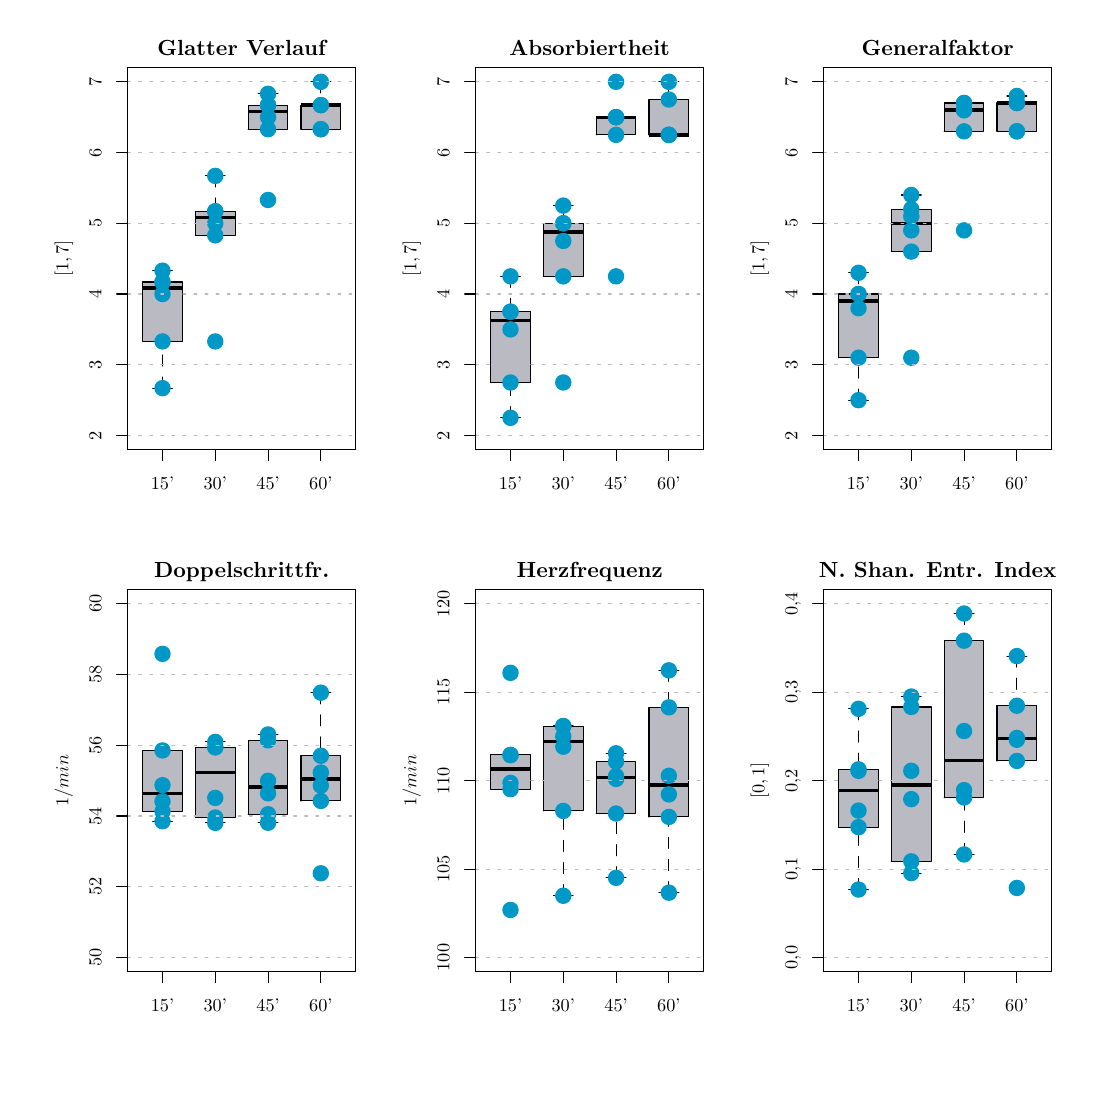
\begin{tikzpicture}[x=1pt,y=1pt]
\definecolor{fillColor}{RGB}{255,255,255}
\path[use as bounding box,fill=fillColor] (0,0) rectangle (377.25,377.25);
\begin{scope}
\path[clip] ( 36.13,224.76) rectangle (118.52,362.80);
\definecolor{fillColor}{RGB}{186,187,194}

\path[fill=fillColor] ( 41.57,263.87) --
	( 55.87,263.87) --
	( 55.87,285.34) --
	( 41.57,285.34) --
	cycle;
\definecolor{drawColor}{RGB}{0,0,0}

\path[draw=drawColor,line width= 1.2pt,line join=round] ( 41.57,283.17) -- ( 55.87,283.17);

\path[draw=drawColor,line width= 0.4pt,dash pattern=on 4pt off 4pt ,line join=round,line cap=round] ( 48.72,247.00) -- ( 48.72,263.87);

\path[draw=drawColor,line width= 0.4pt,dash pattern=on 4pt off 4pt ,line join=round,line cap=round] ( 48.72,289.43) -- ( 48.72,285.34);

\path[draw=drawColor,line width= 0.4pt,line join=round,line cap=round] ( 45.15,247.00) -- ( 52.30,247.00);

\path[draw=drawColor,line width= 0.4pt,line join=round,line cap=round] ( 45.15,289.43) -- ( 52.30,289.43);

\path[draw=drawColor,line width= 0.4pt,line join=round,line cap=round] ( 41.57,263.87) --
	( 55.87,263.87) --
	( 55.87,285.34) --
	( 41.57,285.34) --
	( 41.57,263.87);

\path[fill=fillColor] ( 60.64,302.21) --
	( 74.94,302.21) --
	( 74.94,310.90) --
	( 60.64,310.90) --
	cycle;

\path[draw=drawColor,line width= 1.2pt,line join=round] ( 60.64,308.73) -- ( 74.94,308.73);

\path[draw=drawColor,line width= 0.4pt,dash pattern=on 4pt off 4pt ,line join=round,line cap=round] ( 67.79,302.21) -- ( 67.79,302.21);

\path[draw=drawColor,line width= 0.4pt,dash pattern=on 4pt off 4pt ,line join=round,line cap=round] ( 67.79,323.69) -- ( 67.79,310.90);

\path[draw=drawColor,line width= 0.4pt,line join=round,line cap=round] ( 64.22,302.21) -- ( 71.37,302.21);

\path[draw=drawColor,line width= 0.4pt,line join=round,line cap=round] ( 64.22,323.69) -- ( 71.37,323.69);

\path[draw=drawColor,line width= 0.4pt,line join=round,line cap=round] ( 60.64,302.21) --
	( 74.94,302.21) --
	( 74.94,310.90) --
	( 60.64,310.90) --
	( 60.64,302.21);

\path[fill=fillColor] ( 79.71,340.56) --
	( 94.02,340.56) --
	( 94.02,349.25) --
	( 79.71,349.25) --
	cycle;

\path[draw=drawColor,line width= 1.2pt,line join=round] ( 79.71,347.07) -- ( 94.02,347.07);

\path[draw=drawColor,line width= 0.4pt,dash pattern=on 4pt off 4pt ,line join=round,line cap=round] ( 86.86,340.56) -- ( 86.86,340.56);

\path[draw=drawColor,line width= 0.4pt,dash pattern=on 4pt off 4pt ,line join=round,line cap=round] ( 86.86,353.34) -- ( 86.86,349.25);

\path[draw=drawColor,line width= 0.4pt,line join=round,line cap=round] ( 83.29,340.56) -- ( 90.44,340.56);

\path[draw=drawColor,line width= 0.4pt,line join=round,line cap=round] ( 83.29,353.34) -- ( 90.44,353.34);

\path[draw=drawColor,line width= 0.4pt,line join=round,line cap=round] ( 79.71,340.56) --
	( 94.02,340.56) --
	( 94.02,349.25) --
	( 79.71,349.25) --
	( 79.71,340.56);

\path[fill=fillColor] ( 98.78,340.56) --
	(113.09,340.56) --
	(113.09,349.25) --
	( 98.78,349.25) --
	cycle;

\path[draw=drawColor,line width= 1.2pt,line join=round] ( 98.78,349.25) -- (113.09,349.25);

\path[draw=drawColor,line width= 0.4pt,dash pattern=on 4pt off 4pt ,line join=round,line cap=round] (105.94,340.56) -- (105.94,340.56);

\path[draw=drawColor,line width= 0.4pt,dash pattern=on 4pt off 4pt ,line join=round,line cap=round] (105.94,357.68) -- (105.94,349.25);

\path[draw=drawColor,line width= 0.4pt,line join=round,line cap=round] (102.36,340.56) -- (109.51,340.56);

\path[draw=drawColor,line width= 0.4pt,line join=round,line cap=round] (102.36,357.68) -- (109.51,357.68);

\path[draw=drawColor,line width= 0.4pt,line join=round,line cap=round] ( 98.78,340.56) --
	(113.09,340.56) --
	(113.09,349.25) --
	( 98.78,349.25) --
	( 98.78,340.56);
\end{scope}
\begin{scope}
\path[clip] (  0.00,  0.00) rectangle (377.25,377.25);
\definecolor{drawColor}{RGB}{0,0,0}

\path[draw=drawColor,line width= 0.4pt,line join=round,line cap=round] ( 48.72,224.76) -- (105.94,224.76);

\path[draw=drawColor,line width= 0.4pt,line join=round,line cap=round] ( 48.72,224.76) -- ( 48.72,220.80);

\path[draw=drawColor,line width= 0.4pt,line join=round,line cap=round] ( 67.79,224.76) -- ( 67.79,220.80);

\path[draw=drawColor,line width= 0.4pt,line join=round,line cap=round] ( 86.86,224.76) -- ( 86.86,220.80);

\path[draw=drawColor,line width= 0.4pt,line join=round,line cap=round] (105.94,224.76) -- (105.94,220.80);

\node[text=drawColor,anchor=base,inner sep=0pt, outer sep=0pt, scale=  0.66] at ( 48.72,210.50) {15'};

\node[text=drawColor,anchor=base,inner sep=0pt, outer sep=0pt, scale=  0.66] at ( 67.79,210.50) {30'};

\node[text=drawColor,anchor=base,inner sep=0pt, outer sep=0pt, scale=  0.66] at ( 86.86,210.50) {45'};

\node[text=drawColor,anchor=base,inner sep=0pt, outer sep=0pt, scale=  0.66] at (105.94,210.50) {60'};

\path[draw=drawColor,line width= 0.4pt,line join=round,line cap=round] ( 36.13,229.87) -- ( 36.13,357.68);

\path[draw=drawColor,line width= 0.4pt,line join=round,line cap=round] ( 36.13,229.87) -- ( 32.17,229.87);

\path[draw=drawColor,line width= 0.4pt,line join=round,line cap=round] ( 36.13,255.43) -- ( 32.17,255.43);

\path[draw=drawColor,line width= 0.4pt,line join=round,line cap=round] ( 36.13,281.00) -- ( 32.17,281.00);

\path[draw=drawColor,line width= 0.4pt,line join=round,line cap=round] ( 36.13,306.56) -- ( 32.17,306.56);

\path[draw=drawColor,line width= 0.4pt,line join=round,line cap=round] ( 36.13,332.12) -- ( 32.17,332.12);

\path[draw=drawColor,line width= 0.4pt,line join=round,line cap=round] ( 36.13,357.68) -- ( 32.17,357.68);

\node[text=drawColor,rotate= 90.00,anchor=base,inner sep=0pt, outer sep=0pt, scale=  0.66] at ( 26.63,229.87) {2};

\node[text=drawColor,rotate= 90.00,anchor=base,inner sep=0pt, outer sep=0pt, scale=  0.66] at ( 26.63,255.43) {3};

\node[text=drawColor,rotate= 90.00,anchor=base,inner sep=0pt, outer sep=0pt, scale=  0.66] at ( 26.63,281.00) {4};

\node[text=drawColor,rotate= 90.00,anchor=base,inner sep=0pt, outer sep=0pt, scale=  0.66] at ( 26.63,306.56) {5};

\node[text=drawColor,rotate= 90.00,anchor=base,inner sep=0pt, outer sep=0pt, scale=  0.66] at ( 26.63,332.12) {6};

\node[text=drawColor,rotate= 90.00,anchor=base,inner sep=0pt, outer sep=0pt, scale=  0.66] at ( 26.63,357.68) {7};
\end{scope}
\begin{scope}
\path[clip] (  0.00,188.62) rectangle (125.75,377.25);
\definecolor{drawColor}{RGB}{0,0,0}

\node[text=drawColor,anchor=base,inner sep=0pt, outer sep=0pt, scale=  0.79] at ( 77.33,367.29) {\bfseries Glatter Verlauf};

\node[text=drawColor,rotate= 90.00,anchor=base,inner sep=0pt, outer sep=0pt, scale=  0.66] at ( 14.75,293.78) {$[1, 7]$};
\end{scope}
\begin{scope}
\path[clip] (  0.00,  0.00) rectangle (377.25,377.25);
\definecolor{drawColor}{RGB}{0,0,0}

\path[draw=drawColor,line width= 0.4pt,line join=round,line cap=round] ( 36.13,224.76) --
	(118.52,224.76) --
	(118.52,362.80) --
	( 36.13,362.80) --
	( 36.13,224.76);
\end{scope}
\begin{scope}
\path[clip] ( 36.13,224.76) rectangle (118.52,362.80);
\definecolor{fillColor}{RGB}{0,152,199}

\path[fill=fillColor] ( 48.72,247.00) circle (  2.97);

\path[fill=fillColor] ( 67.79,263.87) circle (  2.97);

\path[fill=fillColor] ( 86.86,314.99) circle (  2.97);

\path[fill=fillColor] (105.94,340.56) circle (  2.97);

\path[fill=fillColor] ( 48.72,263.87) circle (  2.97);

\path[fill=fillColor] ( 67.79,302.21) circle (  2.97);

\path[fill=fillColor] ( 86.86,340.56) circle (  2.97);

\path[fill=fillColor] (105.94,340.56) circle (  2.97);

\path[fill=fillColor] ( 48.72,285.34) circle (  2.97);

\path[fill=fillColor] ( 67.79,323.69) circle (  2.97);

\path[fill=fillColor] ( 86.86,349.25) circle (  2.97);

\path[fill=fillColor] ( 48.72,289.43) circle (  2.97);

\path[fill=fillColor] ( 67.79,310.90) circle (  2.97);

\path[fill=fillColor] ( 86.86,349.25) circle (  2.97);

\path[fill=fillColor] (105.94,349.25) circle (  2.97);

\path[fill=fillColor] ( 48.72,285.34) circle (  2.97);

\path[fill=fillColor] ( 67.79,306.56) circle (  2.97);

\path[fill=fillColor] ( 86.86,353.34) circle (  2.97);

\path[fill=fillColor] (105.94,349.25) circle (  2.97);

\path[fill=fillColor] ( 48.72,281.00) circle (  2.97);

\path[fill=fillColor] ( 67.79,310.90) circle (  2.97);

\path[fill=fillColor] ( 86.86,344.90) circle (  2.97);

\path[fill=fillColor] (105.94,357.68) circle (  2.97);
\definecolor{drawColor}{RGB}{186,187,194}

\path[draw=drawColor,line width= 0.4pt,dash pattern=on 1pt off 3pt ,line join=round,line cap=round] ( 36.13,229.87) -- (118.52,229.87);

\path[draw=drawColor,line width= 0.4pt,dash pattern=on 1pt off 3pt ,line join=round,line cap=round] ( 36.13,255.43) -- (118.52,255.43);

\path[draw=drawColor,line width= 0.4pt,dash pattern=on 1pt off 3pt ,line join=round,line cap=round] ( 36.13,281.00) -- (118.52,281.00);

\path[draw=drawColor,line width= 0.4pt,dash pattern=on 1pt off 3pt ,line join=round,line cap=round] ( 36.13,306.56) -- (118.52,306.56);

\path[draw=drawColor,line width= 0.4pt,dash pattern=on 1pt off 3pt ,line join=round,line cap=round] ( 36.13,332.12) -- (118.52,332.12);

\path[draw=drawColor,line width= 0.4pt,dash pattern=on 1pt off 3pt ,line join=round,line cap=round] ( 36.13,357.68) -- (118.52,357.68);
\end{scope}
\begin{scope}
\path[clip] (  0.00,  0.00) rectangle (377.25,377.25);
\definecolor{drawColor}{RGB}{0,0,0}

\path[draw=drawColor,line width= 0.4pt,line join=round,line cap=round] ( 36.13,224.76) --
	(118.52,224.76) --
	(118.52,362.80) --
	( 36.13,362.80) --
	( 36.13,224.76);
\end{scope}
\begin{scope}
\path[clip] (161.88,224.76) rectangle (244.27,362.80);
\definecolor{fillColor}{RGB}{186,187,194}

\path[fill=fillColor] (167.32,249.04) --
	(181.62,249.04) --
	(181.62,274.61) --
	(167.32,274.61) --
	cycle;
\definecolor{drawColor}{RGB}{0,0,0}

\path[draw=drawColor,line width= 1.2pt,line join=round] (167.32,271.41) -- (181.62,271.41);

\path[draw=drawColor,line width= 0.4pt,dash pattern=on 4pt off 4pt ,line join=round,line cap=round] (174.47,236.26) -- (174.47,249.04);

\path[draw=drawColor,line width= 0.4pt,dash pattern=on 4pt off 4pt ,line join=round,line cap=round] (174.47,287.39) -- (174.47,274.61);

\path[draw=drawColor,line width= 0.4pt,line join=round,line cap=round] (170.90,236.26) -- (178.05,236.26);

\path[draw=drawColor,line width= 0.4pt,line join=round,line cap=round] (170.90,287.39) -- (178.05,287.39);

\path[draw=drawColor,line width= 0.4pt,line join=round,line cap=round] (167.32,249.04) --
	(181.62,249.04) --
	(181.62,274.61) --
	(167.32,274.61) --
	(167.32,249.04);

\path[fill=fillColor] (186.39,287.39) --
	(200.69,287.39) --
	(200.69,306.56) --
	(186.39,306.56) --
	cycle;

\path[draw=drawColor,line width= 1.2pt,line join=round] (186.39,303.36) -- (200.69,303.36);

\path[draw=drawColor,line width= 0.4pt,dash pattern=on 4pt off 4pt ,line join=round,line cap=round] (193.54,287.39) -- (193.54,287.39);

\path[draw=drawColor,line width= 0.4pt,dash pattern=on 4pt off 4pt ,line join=round,line cap=round] (193.54,312.95) -- (193.54,306.56);

\path[draw=drawColor,line width= 0.4pt,line join=round,line cap=round] (189.97,287.39) -- (197.12,287.39);

\path[draw=drawColor,line width= 0.4pt,line join=round,line cap=round] (189.97,312.95) -- (197.12,312.95);

\path[draw=drawColor,line width= 0.4pt,line join=round,line cap=round] (186.39,287.39) --
	(200.69,287.39) --
	(200.69,306.56) --
	(186.39,306.56) --
	(186.39,287.39);

\path[fill=fillColor] (205.46,338.51) --
	(219.77,338.51) --
	(219.77,344.90) --
	(205.46,344.90) --
	cycle;

\path[draw=drawColor,line width= 1.2pt,line join=round] (205.46,344.90) -- (219.77,344.90);

\path[draw=drawColor,line width= 0.4pt,dash pattern=on 4pt off 4pt ,line join=round,line cap=round] (212.61,338.51) -- (212.61,338.51);

\path[draw=drawColor,line width= 0.4pt,dash pattern=on 4pt off 4pt ,line join=round,line cap=round] (212.61,344.90) -- (212.61,344.90);

\path[draw=drawColor,line width= 0.4pt,line join=round,line cap=round] (209.04,338.51) -- (216.19,338.51);

\path[draw=drawColor,line width= 0.4pt,line join=round,line cap=round] (209.04,344.90) -- (216.19,344.90);

\path[draw=drawColor,line width= 0.4pt,line join=round,line cap=round] (205.46,338.51) --
	(219.77,338.51) --
	(219.77,344.90) --
	(205.46,344.90) --
	(205.46,338.51);

\path[fill=fillColor] (224.53,338.51) --
	(238.84,338.51) --
	(238.84,351.29) --
	(224.53,351.29) --
	cycle;

\path[draw=drawColor,line width= 1.2pt,line join=round] (224.53,338.51) -- (238.84,338.51);

\path[draw=drawColor,line width= 0.4pt,dash pattern=on 4pt off 4pt ,line join=round,line cap=round] (231.69,338.51) -- (231.69,338.51);

\path[draw=drawColor,line width= 0.4pt,dash pattern=on 4pt off 4pt ,line join=round,line cap=round] (231.69,357.68) -- (231.69,351.29);

\path[draw=drawColor,line width= 0.4pt,line join=round,line cap=round] (228.11,338.51) -- (235.26,338.51);

\path[draw=drawColor,line width= 0.4pt,line join=round,line cap=round] (228.11,357.68) -- (235.26,357.68);

\path[draw=drawColor,line width= 0.4pt,line join=round,line cap=round] (224.53,338.51) --
	(238.84,338.51) --
	(238.84,351.29) --
	(224.53,351.29) --
	(224.53,338.51);
\end{scope}
\begin{scope}
\path[clip] (  0.00,  0.00) rectangle (377.25,377.25);
\definecolor{drawColor}{RGB}{0,0,0}

\path[draw=drawColor,line width= 0.4pt,line join=round,line cap=round] (174.47,224.76) -- (231.69,224.76);

\path[draw=drawColor,line width= 0.4pt,line join=round,line cap=round] (174.47,224.76) -- (174.47,220.80);

\path[draw=drawColor,line width= 0.4pt,line join=round,line cap=round] (193.54,224.76) -- (193.54,220.80);

\path[draw=drawColor,line width= 0.4pt,line join=round,line cap=round] (212.61,224.76) -- (212.61,220.80);

\path[draw=drawColor,line width= 0.4pt,line join=round,line cap=round] (231.69,224.76) -- (231.69,220.80);

\node[text=drawColor,anchor=base,inner sep=0pt, outer sep=0pt, scale=  0.66] at (174.47,210.50) {15'};

\node[text=drawColor,anchor=base,inner sep=0pt, outer sep=0pt, scale=  0.66] at (193.54,210.50) {30'};

\node[text=drawColor,anchor=base,inner sep=0pt, outer sep=0pt, scale=  0.66] at (212.61,210.50) {45'};

\node[text=drawColor,anchor=base,inner sep=0pt, outer sep=0pt, scale=  0.66] at (231.69,210.50) {60'};

\path[draw=drawColor,line width= 0.4pt,line join=round,line cap=round] (161.88,229.87) -- (161.88,357.68);

\path[draw=drawColor,line width= 0.4pt,line join=round,line cap=round] (161.88,229.87) -- (157.92,229.87);

\path[draw=drawColor,line width= 0.4pt,line join=round,line cap=round] (161.88,255.43) -- (157.92,255.43);

\path[draw=drawColor,line width= 0.4pt,line join=round,line cap=round] (161.88,281.00) -- (157.92,281.00);

\path[draw=drawColor,line width= 0.4pt,line join=round,line cap=round] (161.88,306.56) -- (157.92,306.56);

\path[draw=drawColor,line width= 0.4pt,line join=round,line cap=round] (161.88,332.12) -- (157.92,332.12);

\path[draw=drawColor,line width= 0.4pt,line join=round,line cap=round] (161.88,357.68) -- (157.92,357.68);

\node[text=drawColor,rotate= 90.00,anchor=base,inner sep=0pt, outer sep=0pt, scale=  0.66] at (152.38,229.87) {2};

\node[text=drawColor,rotate= 90.00,anchor=base,inner sep=0pt, outer sep=0pt, scale=  0.66] at (152.38,255.43) {3};

\node[text=drawColor,rotate= 90.00,anchor=base,inner sep=0pt, outer sep=0pt, scale=  0.66] at (152.38,281.00) {4};

\node[text=drawColor,rotate= 90.00,anchor=base,inner sep=0pt, outer sep=0pt, scale=  0.66] at (152.38,306.56) {5};

\node[text=drawColor,rotate= 90.00,anchor=base,inner sep=0pt, outer sep=0pt, scale=  0.66] at (152.38,332.12) {6};

\node[text=drawColor,rotate= 90.00,anchor=base,inner sep=0pt, outer sep=0pt, scale=  0.66] at (152.38,357.68) {7};
\end{scope}
\begin{scope}
\path[clip] (125.75,188.62) rectangle (251.50,377.25);
\definecolor{drawColor}{RGB}{0,0,0}

\node[text=drawColor,anchor=base,inner sep=0pt, outer sep=0pt, scale=  0.79] at (203.08,367.29) {\bfseries Absorbiertheit};

\node[text=drawColor,rotate= 90.00,anchor=base,inner sep=0pt, outer sep=0pt, scale=  0.66] at (140.50,293.78) {$[1, 7]$};
\end{scope}
\begin{scope}
\path[clip] (  0.00,  0.00) rectangle (377.25,377.25);
\definecolor{drawColor}{RGB}{0,0,0}

\path[draw=drawColor,line width= 0.4pt,line join=round,line cap=round] (161.88,224.76) --
	(244.27,224.76) --
	(244.27,362.80) --
	(161.88,362.80) --
	(161.88,224.76);
\end{scope}
\begin{scope}
\path[clip] (161.88,224.76) rectangle (244.27,362.80);
\definecolor{fillColor}{RGB}{0,152,199}

\path[fill=fillColor] (174.47,236.26) circle (  2.97);

\path[fill=fillColor] (193.54,249.04) circle (  2.97);

\path[fill=fillColor] (212.61,287.39) circle (  2.97);

\path[fill=fillColor] (231.69,338.51) circle (  2.97);

\path[fill=fillColor] (174.47,249.04) circle (  2.97);

\path[fill=fillColor] (193.54,287.39) circle (  2.97);

\path[fill=fillColor] (212.61,338.51) circle (  2.97);

\path[fill=fillColor] (231.69,338.51) circle (  2.97);

\path[fill=fillColor] (174.47,274.61) circle (  2.97);

\path[fill=fillColor] (193.54,306.56) circle (  2.97);

\path[fill=fillColor] (212.61,344.90) circle (  2.97);

\path[fill=fillColor] (174.47,287.39) circle (  2.97);

\path[fill=fillColor] (193.54,312.95) circle (  2.97);

\path[fill=fillColor] (212.61,344.90) circle (  2.97);

\path[fill=fillColor] (231.69,351.29) circle (  2.97);

\path[fill=fillColor] (174.47,274.61) circle (  2.97);

\path[fill=fillColor] (193.54,300.17) circle (  2.97);

\path[fill=fillColor] (212.61,344.90) circle (  2.97);

\path[fill=fillColor] (231.69,357.68) circle (  2.97);

\path[fill=fillColor] (174.47,268.22) circle (  2.97);

\path[fill=fillColor] (193.54,306.56) circle (  2.97);

\path[fill=fillColor] (212.61,357.68) circle (  2.97);

\path[fill=fillColor] (231.69,338.51) circle (  2.97);
\definecolor{drawColor}{RGB}{186,187,194}

\path[draw=drawColor,line width= 0.4pt,dash pattern=on 1pt off 3pt ,line join=round,line cap=round] (161.88,229.87) -- (244.27,229.87);

\path[draw=drawColor,line width= 0.4pt,dash pattern=on 1pt off 3pt ,line join=round,line cap=round] (161.88,255.43) -- (244.27,255.43);

\path[draw=drawColor,line width= 0.4pt,dash pattern=on 1pt off 3pt ,line join=round,line cap=round] (161.88,281.00) -- (244.27,281.00);

\path[draw=drawColor,line width= 0.4pt,dash pattern=on 1pt off 3pt ,line join=round,line cap=round] (161.88,306.56) -- (244.27,306.56);

\path[draw=drawColor,line width= 0.4pt,dash pattern=on 1pt off 3pt ,line join=round,line cap=round] (161.88,332.12) -- (244.27,332.12);

\path[draw=drawColor,line width= 0.4pt,dash pattern=on 1pt off 3pt ,line join=round,line cap=round] (161.88,357.68) -- (244.27,357.68);
\end{scope}
\begin{scope}
\path[clip] (  0.00,  0.00) rectangle (377.25,377.25);
\definecolor{drawColor}{RGB}{0,0,0}

\path[draw=drawColor,line width= 0.4pt,line join=round,line cap=round] (161.88,224.76) --
	(244.27,224.76) --
	(244.27,362.80) --
	(161.88,362.80) --
	(161.88,224.76);
\end{scope}
\begin{scope}
\path[clip] (287.63,224.76) rectangle (370.02,362.80);
\definecolor{fillColor}{RGB}{186,187,194}

\path[fill=fillColor] (293.07,257.99) --
	(307.37,257.99) --
	(307.37,281.00) --
	(293.07,281.00) --
	cycle;
\definecolor{drawColor}{RGB}{0,0,0}

\path[draw=drawColor,line width= 1.2pt,line join=round] (293.07,278.44) -- (307.37,278.44);

\path[draw=drawColor,line width= 0.4pt,dash pattern=on 4pt off 4pt ,line join=round,line cap=round] (300.22,242.65) -- (300.22,257.99);

\path[draw=drawColor,line width= 0.4pt,dash pattern=on 4pt off 4pt ,line join=round,line cap=round] (300.22,288.67) -- (300.22,281.00);

\path[draw=drawColor,line width= 0.4pt,line join=round,line cap=round] (296.65,242.65) -- (303.80,242.65);

\path[draw=drawColor,line width= 0.4pt,line join=round,line cap=round] (296.65,288.67) -- (303.80,288.67);

\path[draw=drawColor,line width= 0.4pt,line join=round,line cap=round] (293.07,257.99) --
	(307.37,257.99) --
	(307.37,281.00) --
	(293.07,281.00) --
	(293.07,257.99);

\path[fill=fillColor] (312.14,296.33) --
	(326.44,296.33) --
	(326.44,311.67) --
	(312.14,311.67) --
	cycle;

\path[draw=drawColor,line width= 1.2pt,line join=round] (312.14,306.56) -- (326.44,306.56);

\path[draw=drawColor,line width= 0.4pt,dash pattern=on 4pt off 4pt ,line join=round,line cap=round] (319.29,296.33) -- (319.29,296.33);

\path[draw=drawColor,line width= 0.4pt,dash pattern=on 4pt off 4pt ,line join=round,line cap=round] (319.29,316.78) -- (319.29,311.67);

\path[draw=drawColor,line width= 0.4pt,line join=round,line cap=round] (315.72,296.33) -- (322.87,296.33);

\path[draw=drawColor,line width= 0.4pt,line join=round,line cap=round] (315.72,316.78) -- (322.87,316.78);

\path[draw=drawColor,line width= 0.4pt,line join=round,line cap=round] (312.14,296.33) --
	(326.44,296.33) --
	(326.44,311.67) --
	(312.14,311.67) --
	(312.14,296.33);

\path[fill=fillColor] (331.21,339.79) --
	(345.52,339.79) --
	(345.52,350.01) --
	(331.21,350.01) --
	cycle;

\path[draw=drawColor,line width= 1.2pt,line join=round] (331.21,347.46) -- (345.52,347.46);

\path[draw=drawColor,line width= 0.4pt,dash pattern=on 4pt off 4pt ,line join=round,line cap=round] (338.36,339.79) -- (338.36,339.79);

\path[draw=drawColor,line width= 0.4pt,dash pattern=on 4pt off 4pt ,line join=round,line cap=round] (338.36,350.01) -- (338.36,350.01);

\path[draw=drawColor,line width= 0.4pt,line join=round,line cap=round] (334.79,339.79) -- (341.94,339.79);

\path[draw=drawColor,line width= 0.4pt,line join=round,line cap=round] (334.79,350.01) -- (341.94,350.01);

\path[draw=drawColor,line width= 0.4pt,line join=round,line cap=round] (331.21,339.79) --
	(345.52,339.79) --
	(345.52,350.01) --
	(331.21,350.01) --
	(331.21,339.79);

\path[fill=fillColor] (350.28,339.79) --
	(364.59,339.79) --
	(364.59,350.01) --
	(350.28,350.01) --
	cycle;

\path[draw=drawColor,line width= 1.2pt,line join=round] (350.28,350.01) -- (364.59,350.01);

\path[draw=drawColor,line width= 0.4pt,dash pattern=on 4pt off 4pt ,line join=round,line cap=round] (357.44,339.79) -- (357.44,339.79);

\path[draw=drawColor,line width= 0.4pt,dash pattern=on 4pt off 4pt ,line join=round,line cap=round] (357.44,352.57) -- (357.44,350.01);

\path[draw=drawColor,line width= 0.4pt,line join=round,line cap=round] (353.86,339.79) -- (361.01,339.79);

\path[draw=drawColor,line width= 0.4pt,line join=round,line cap=round] (353.86,352.57) -- (361.01,352.57);

\path[draw=drawColor,line width= 0.4pt,line join=round,line cap=round] (350.28,339.79) --
	(364.59,339.79) --
	(364.59,350.01) --
	(350.28,350.01) --
	(350.28,339.79);
\end{scope}
\begin{scope}
\path[clip] (  0.00,  0.00) rectangle (377.25,377.25);
\definecolor{drawColor}{RGB}{0,0,0}

\path[draw=drawColor,line width= 0.4pt,line join=round,line cap=round] (300.22,224.76) -- (357.44,224.76);

\path[draw=drawColor,line width= 0.4pt,line join=round,line cap=round] (300.22,224.76) -- (300.22,220.80);

\path[draw=drawColor,line width= 0.4pt,line join=round,line cap=round] (319.29,224.76) -- (319.29,220.80);

\path[draw=drawColor,line width= 0.4pt,line join=round,line cap=round] (338.36,224.76) -- (338.36,220.80);

\path[draw=drawColor,line width= 0.4pt,line join=round,line cap=round] (357.44,224.76) -- (357.44,220.80);

\node[text=drawColor,anchor=base,inner sep=0pt, outer sep=0pt, scale=  0.66] at (300.22,210.50) {15'};

\node[text=drawColor,anchor=base,inner sep=0pt, outer sep=0pt, scale=  0.66] at (319.29,210.50) {30'};

\node[text=drawColor,anchor=base,inner sep=0pt, outer sep=0pt, scale=  0.66] at (338.36,210.50) {45'};

\node[text=drawColor,anchor=base,inner sep=0pt, outer sep=0pt, scale=  0.66] at (357.44,210.50) {60'};

\path[draw=drawColor,line width= 0.4pt,line join=round,line cap=round] (287.63,229.87) -- (287.63,357.68);

\path[draw=drawColor,line width= 0.4pt,line join=round,line cap=round] (287.63,229.87) -- (283.67,229.87);

\path[draw=drawColor,line width= 0.4pt,line join=round,line cap=round] (287.63,255.43) -- (283.67,255.43);

\path[draw=drawColor,line width= 0.4pt,line join=round,line cap=round] (287.63,281.00) -- (283.67,281.00);

\path[draw=drawColor,line width= 0.4pt,line join=round,line cap=round] (287.63,306.56) -- (283.67,306.56);

\path[draw=drawColor,line width= 0.4pt,line join=round,line cap=round] (287.63,332.12) -- (283.67,332.12);

\path[draw=drawColor,line width= 0.4pt,line join=round,line cap=round] (287.63,357.68) -- (283.67,357.68);

\node[text=drawColor,rotate= 90.00,anchor=base,inner sep=0pt, outer sep=0pt, scale=  0.66] at (278.13,229.87) {2};

\node[text=drawColor,rotate= 90.00,anchor=base,inner sep=0pt, outer sep=0pt, scale=  0.66] at (278.13,255.43) {3};

\node[text=drawColor,rotate= 90.00,anchor=base,inner sep=0pt, outer sep=0pt, scale=  0.66] at (278.13,281.00) {4};

\node[text=drawColor,rotate= 90.00,anchor=base,inner sep=0pt, outer sep=0pt, scale=  0.66] at (278.13,306.56) {5};

\node[text=drawColor,rotate= 90.00,anchor=base,inner sep=0pt, outer sep=0pt, scale=  0.66] at (278.13,332.12) {6};

\node[text=drawColor,rotate= 90.00,anchor=base,inner sep=0pt, outer sep=0pt, scale=  0.66] at (278.13,357.68) {7};
\end{scope}
\begin{scope}
\path[clip] (251.50,188.62) rectangle (377.25,377.25);
\definecolor{drawColor}{RGB}{0,0,0}

\node[text=drawColor,anchor=base,inner sep=0pt, outer sep=0pt, scale=  0.79] at (328.83,367.29) {\bfseries Generalfaktor};

\node[text=drawColor,rotate= 90.00,anchor=base,inner sep=0pt, outer sep=0pt, scale=  0.66] at (266.25,293.78) {$[1, 7]$};
\end{scope}
\begin{scope}
\path[clip] (  0.00,  0.00) rectangle (377.25,377.25);
\definecolor{drawColor}{RGB}{0,0,0}

\path[draw=drawColor,line width= 0.4pt,line join=round,line cap=round] (287.63,224.76) --
	(370.02,224.76) --
	(370.02,362.80) --
	(287.63,362.80) --
	(287.63,224.76);
\end{scope}
\begin{scope}
\path[clip] (287.63,224.76) rectangle (370.02,362.80);
\definecolor{fillColor}{RGB}{0,152,199}

\path[fill=fillColor] (300.22,242.65) circle (  2.97);

\path[fill=fillColor] (319.29,257.99) circle (  2.97);

\path[fill=fillColor] (338.36,304.00) circle (  2.97);

\path[fill=fillColor] (357.44,339.79) circle (  2.97);

\path[fill=fillColor] (300.22,257.99) circle (  2.97);

\path[fill=fillColor] (319.29,296.33) circle (  2.97);

\path[fill=fillColor] (338.36,339.79) circle (  2.97);

\path[fill=fillColor] (357.44,339.79) circle (  2.97);

\path[fill=fillColor] (300.22,281.00) circle (  2.97);

\path[fill=fillColor] (319.29,316.78) circle (  2.97);

\path[fill=fillColor] (338.36,347.46) circle (  2.97);

\path[fill=fillColor] (300.22,288.67) circle (  2.97);

\path[fill=fillColor] (319.29,311.67) circle (  2.97);

\path[fill=fillColor] (338.36,347.46) circle (  2.97);

\path[fill=fillColor] (357.44,350.01) circle (  2.97);

\path[fill=fillColor] (300.22,281.00) circle (  2.97);

\path[fill=fillColor] (319.29,304.00) circle (  2.97);

\path[fill=fillColor] (338.36,350.01) circle (  2.97);

\path[fill=fillColor] (357.44,352.57) circle (  2.97);

\path[fill=fillColor] (300.22,275.88) circle (  2.97);

\path[fill=fillColor] (319.29,309.11) circle (  2.97);

\path[fill=fillColor] (338.36,350.01) circle (  2.97);

\path[fill=fillColor] (357.44,350.01) circle (  2.97);
\definecolor{drawColor}{RGB}{186,187,194}

\path[draw=drawColor,line width= 0.4pt,dash pattern=on 1pt off 3pt ,line join=round,line cap=round] (287.63,229.87) -- (370.02,229.87);

\path[draw=drawColor,line width= 0.4pt,dash pattern=on 1pt off 3pt ,line join=round,line cap=round] (287.63,255.43) -- (370.02,255.43);

\path[draw=drawColor,line width= 0.4pt,dash pattern=on 1pt off 3pt ,line join=round,line cap=round] (287.63,281.00) -- (370.02,281.00);

\path[draw=drawColor,line width= 0.4pt,dash pattern=on 1pt off 3pt ,line join=round,line cap=round] (287.63,306.56) -- (370.02,306.56);

\path[draw=drawColor,line width= 0.4pt,dash pattern=on 1pt off 3pt ,line join=round,line cap=round] (287.63,332.12) -- (370.02,332.12);

\path[draw=drawColor,line width= 0.4pt,dash pattern=on 1pt off 3pt ,line join=round,line cap=round] (287.63,357.68) -- (370.02,357.68);
\end{scope}
\begin{scope}
\path[clip] (  0.00,  0.00) rectangle (377.25,377.25);
\definecolor{drawColor}{RGB}{0,0,0}

\path[draw=drawColor,line width= 0.4pt,line join=round,line cap=round] (287.63,224.76) --
	(370.02,224.76) --
	(370.02,362.80) --
	(287.63,362.80) --
	(287.63,224.76);
\end{scope}
\begin{scope}
\path[clip] ( 36.13, 36.13) rectangle (118.52,174.17);
\definecolor{fillColor}{RGB}{186,187,194}

\path[fill=fillColor] ( 41.57, 94.06) --
	( 55.87, 94.06) --
	( 55.87,116.08) --
	( 41.57,116.08) --
	cycle;
\definecolor{drawColor}{RGB}{0,0,0}

\path[draw=drawColor,line width= 1.2pt,line join=round] ( 41.57,100.60) -- ( 55.87,100.60);

\path[draw=drawColor,line width= 0.4pt,dash pattern=on 4pt off 4pt ,line join=round,line cap=round] ( 48.72, 90.50) -- ( 48.72, 94.06);

\path[draw=drawColor,line width= 0.4pt,dash pattern=on 4pt off 4pt ,line join=round,line cap=round] ( 48.72,116.08) -- ( 48.72,116.08);

\path[draw=drawColor,line width= 0.4pt,line join=round,line cap=round] ( 45.15, 90.50) -- ( 52.30, 90.50);

\path[draw=drawColor,line width= 0.4pt,line join=round,line cap=round] ( 45.15,116.08) -- ( 52.30,116.08);

\path[draw=drawColor,line width= 0.4pt,line join=round,line cap=round] ( 41.57, 94.06) --
	( 55.87, 94.06) --
	( 55.87,116.08) --
	( 41.57,116.08) --
	( 41.57, 94.06);

\path[fill=fillColor] ( 60.64, 91.83) --
	( 74.94, 91.83) --
	( 74.94,117.29) --
	( 60.64,117.29) --
	cycle;

\path[draw=drawColor,line width= 1.2pt,line join=round] ( 60.64,108.05) -- ( 74.94,108.05);

\path[draw=drawColor,line width= 0.4pt,dash pattern=on 4pt off 4pt ,line join=round,line cap=round] ( 67.79, 89.90) -- ( 67.79, 91.83);

\path[draw=drawColor,line width= 0.4pt,dash pattern=on 4pt off 4pt ,line join=round,line cap=round] ( 67.79,119.17) -- ( 67.79,117.29);

\path[draw=drawColor,line width= 0.4pt,line join=round,line cap=round] ( 64.22, 89.90) -- ( 71.37, 89.90);

\path[draw=drawColor,line width= 0.4pt,line join=round,line cap=round] ( 64.22,119.17) -- ( 71.37,119.17);

\path[draw=drawColor,line width= 0.4pt,line join=round,line cap=round] ( 60.64, 91.83) --
	( 74.94, 91.83) --
	( 74.94,117.29) --
	( 60.64,117.29) --
	( 60.64, 91.83);

\path[fill=fillColor] ( 79.71, 93.01) --
	( 94.02, 93.01) --
	( 94.02,119.72) --
	( 79.71,119.72) --
	cycle;

\path[draw=drawColor,line width= 1.2pt,line join=round] ( 79.71,102.84) -- ( 94.02,102.84);

\path[draw=drawColor,line width= 0.4pt,dash pattern=on 4pt off 4pt ,line join=round,line cap=round] ( 86.86, 89.94) -- ( 86.86, 93.01);

\path[draw=drawColor,line width= 0.4pt,dash pattern=on 4pt off 4pt ,line join=round,line cap=round] ( 86.86,121.85) -- ( 86.86,119.72);

\path[draw=drawColor,line width= 0.4pt,line join=round,line cap=round] ( 83.29, 89.94) -- ( 90.44, 89.94);

\path[draw=drawColor,line width= 0.4pt,line join=round,line cap=round] ( 83.29,121.85) -- ( 90.44,121.85);

\path[draw=drawColor,line width= 0.4pt,line join=round,line cap=round] ( 79.71, 93.01) --
	( 94.02, 93.01) --
	( 94.02,119.72) --
	( 79.71,119.72) --
	( 79.71, 93.01);

\path[fill=fillColor] ( 98.78, 97.83) --
	(113.09, 97.83) --
	(113.09,114.15) --
	( 98.78,114.15) --
	cycle;

\path[draw=drawColor,line width= 1.2pt,line join=round] ( 98.78,105.74) -- (113.09,105.74);

\path[draw=drawColor,line width= 0.4pt,dash pattern=on 4pt off 4pt ,line join=round,line cap=round] (105.94, 97.83) -- (105.94, 97.83);

\path[draw=drawColor,line width= 0.4pt,dash pattern=on 4pt off 4pt ,line join=round,line cap=round] (105.94,136.95) -- (105.94,114.15);

\path[draw=drawColor,line width= 0.4pt,line join=round,line cap=round] (102.36, 97.83) -- (109.51, 97.83);

\path[draw=drawColor,line width= 0.4pt,line join=round,line cap=round] (102.36,136.95) -- (109.51,136.95);

\path[draw=drawColor,line width= 0.4pt,line join=round,line cap=round] ( 98.78, 97.83) --
	(113.09, 97.83) --
	(113.09,114.15) --
	( 98.78,114.15) --
	( 98.78, 97.83);
\end{scope}
\begin{scope}
\path[clip] (  0.00,  0.00) rectangle (377.25,377.25);
\definecolor{drawColor}{RGB}{0,0,0}

\path[draw=drawColor,line width= 0.4pt,line join=round,line cap=round] ( 48.72, 36.13) -- (105.94, 36.13);

\path[draw=drawColor,line width= 0.4pt,line join=round,line cap=round] ( 48.72, 36.13) -- ( 48.72, 32.17);

\path[draw=drawColor,line width= 0.4pt,line join=round,line cap=round] ( 67.79, 36.13) -- ( 67.79, 32.17);

\path[draw=drawColor,line width= 0.4pt,line join=round,line cap=round] ( 86.86, 36.13) -- ( 86.86, 32.17);

\path[draw=drawColor,line width= 0.4pt,line join=round,line cap=round] (105.94, 36.13) -- (105.94, 32.17);

\node[text=drawColor,anchor=base,inner sep=0pt, outer sep=0pt, scale=  0.66] at ( 48.72, 21.88) {15'};

\node[text=drawColor,anchor=base,inner sep=0pt, outer sep=0pt, scale=  0.66] at ( 67.79, 21.88) {30'};

\node[text=drawColor,anchor=base,inner sep=0pt, outer sep=0pt, scale=  0.66] at ( 86.86, 21.88) {45'};

\node[text=drawColor,anchor=base,inner sep=0pt, outer sep=0pt, scale=  0.66] at (105.94, 21.88) {60'};

\path[draw=drawColor,line width= 0.4pt,line join=round,line cap=round] ( 36.13, 41.25) -- ( 36.13,169.06);

\path[draw=drawColor,line width= 0.4pt,line join=round,line cap=round] ( 36.13, 41.25) -- ( 32.17, 41.25);

\path[draw=drawColor,line width= 0.4pt,line join=round,line cap=round] ( 36.13, 66.81) -- ( 32.17, 66.81);

\path[draw=drawColor,line width= 0.4pt,line join=round,line cap=round] ( 36.13, 92.37) -- ( 32.17, 92.37);

\path[draw=drawColor,line width= 0.4pt,line join=round,line cap=round] ( 36.13,117.93) -- ( 32.17,117.93);

\path[draw=drawColor,line width= 0.4pt,line join=round,line cap=round] ( 36.13,143.50) -- ( 32.17,143.50);

\path[draw=drawColor,line width= 0.4pt,line join=round,line cap=round] ( 36.13,169.06) -- ( 32.17,169.06);

\node[text=drawColor,rotate= 90.00,anchor=base,inner sep=0pt, outer sep=0pt, scale=  0.66] at ( 26.63, 41.25) {50};

\node[text=drawColor,rotate= 90.00,anchor=base,inner sep=0pt, outer sep=0pt, scale=  0.66] at ( 26.63, 66.81) {52};

\node[text=drawColor,rotate= 90.00,anchor=base,inner sep=0pt, outer sep=0pt, scale=  0.66] at ( 26.63, 92.37) {54};

\node[text=drawColor,rotate= 90.00,anchor=base,inner sep=0pt, outer sep=0pt, scale=  0.66] at ( 26.63,117.93) {56};

\node[text=drawColor,rotate= 90.00,anchor=base,inner sep=0pt, outer sep=0pt, scale=  0.66] at ( 26.63,143.50) {58};

\node[text=drawColor,rotate= 90.00,anchor=base,inner sep=0pt, outer sep=0pt, scale=  0.66] at ( 26.63,169.06) {60};
\end{scope}
\begin{scope}
\path[clip] (  0.00,  0.00) rectangle (125.75,188.62);
\definecolor{drawColor}{RGB}{0,0,0}

\node[text=drawColor,anchor=base,inner sep=0pt, outer sep=0pt, scale=  0.79] at ( 77.33,178.66) {\bfseries Doppelschrittfr.};

\node[text=drawColor,rotate= 90.00,anchor=base,inner sep=0pt, outer sep=0pt, scale=  0.66] at ( 14.75,105.15) {$1/min$};
\end{scope}
\begin{scope}
\path[clip] (  0.00,  0.00) rectangle (377.25,377.25);
\definecolor{drawColor}{RGB}{0,0,0}

\path[draw=drawColor,line width= 0.4pt,line join=round,line cap=round] ( 36.13, 36.13) --
	(118.52, 36.13) --
	(118.52,174.17) --
	( 36.13,174.17) --
	( 36.13, 36.13);
\end{scope}
\begin{scope}
\path[clip] ( 36.13, 36.13) rectangle (118.52,174.17);
\definecolor{fillColor}{RGB}{0,152,199}

\path[fill=fillColor] ( 48.72, 94.06) circle (  2.97);

\path[fill=fillColor] ( 67.79,117.17) circle (  2.97);

\path[fill=fillColor] ( 86.86,100.58) circle (  2.97);

\path[fill=fillColor] (105.94,103.37) circle (  2.97);

\path[fill=fillColor] ( 48.72,116.08) circle (  2.97);

\path[fill=fillColor] ( 67.79,117.29) circle (  2.97);

\path[fill=fillColor] ( 86.86,105.10) circle (  2.97);

\path[fill=fillColor] (105.94, 97.83) circle (  2.97);

\path[fill=fillColor] ( 48.72,150.97) circle (  2.97);

\path[fill=fillColor] ( 67.79,119.17) circle (  2.97);

\path[fill=fillColor] ( 86.86,119.72) circle (  2.97);

\path[fill=fillColor] (105.94,136.95) circle (  2.97);

\path[fill=fillColor] ( 48.72, 90.50) circle (  2.97);

\path[fill=fillColor] ( 67.79, 89.90) circle (  2.97);

\path[fill=fillColor] ( 86.86, 93.01) circle (  2.97);

\path[fill=fillColor] (105.94, 71.69) circle (  2.97);

\path[fill=fillColor] ( 48.72,103.54) circle (  2.97);

\path[fill=fillColor] ( 67.79, 91.83) circle (  2.97);

\path[fill=fillColor] ( 86.86, 89.94) circle (  2.97);

\path[fill=fillColor] (105.94,108.10) circle (  2.97);

\path[fill=fillColor] ( 48.72, 97.66) circle (  2.97);

\path[fill=fillColor] ( 67.79, 98.92) circle (  2.97);

\path[fill=fillColor] ( 86.86,121.85) circle (  2.97);

\path[fill=fillColor] (105.94,114.15) circle (  2.97);
\definecolor{drawColor}{RGB}{186,187,194}

\path[draw=drawColor,line width= 0.4pt,dash pattern=on 1pt off 3pt ,line join=round,line cap=round] ( 36.13, 41.25) -- (118.52, 41.25);

\path[draw=drawColor,line width= 0.4pt,dash pattern=on 1pt off 3pt ,line join=round,line cap=round] ( 36.13, 66.81) -- (118.52, 66.81);

\path[draw=drawColor,line width= 0.4pt,dash pattern=on 1pt off 3pt ,line join=round,line cap=round] ( 36.13, 92.37) -- (118.52, 92.37);

\path[draw=drawColor,line width= 0.4pt,dash pattern=on 1pt off 3pt ,line join=round,line cap=round] ( 36.13,117.93) -- (118.52,117.93);

\path[draw=drawColor,line width= 0.4pt,dash pattern=on 1pt off 3pt ,line join=round,line cap=round] ( 36.13,143.50) -- (118.52,143.50);

\path[draw=drawColor,line width= 0.4pt,dash pattern=on 1pt off 3pt ,line join=round,line cap=round] ( 36.13,169.06) -- (118.52,169.06);
\end{scope}
\begin{scope}
\path[clip] (  0.00,  0.00) rectangle (377.25,377.25);
\definecolor{drawColor}{RGB}{0,0,0}

\path[draw=drawColor,line width= 0.4pt,line join=round,line cap=round] ( 36.13, 36.13) --
	(118.52, 36.13) --
	(118.52,174.17) --
	( 36.13,174.17) --
	( 36.13, 36.13);
\end{scope}
\begin{scope}
\path[clip] (161.88, 36.13) rectangle (244.27,174.17);
\definecolor{fillColor}{RGB}{186,187,194}

\path[fill=fillColor] (167.32,102.09) --
	(181.62,102.09) --
	(181.62,114.46) --
	(167.32,114.46) --
	cycle;
\definecolor{drawColor}{RGB}{0,0,0}

\path[draw=drawColor,line width= 1.2pt,line join=round] (167.32,109.35) -- (181.62,109.35);

\path[draw=drawColor,line width= 0.4pt,dash pattern=on 4pt off 4pt ,line join=round,line cap=round] (174.47,102.09) -- (174.47,102.09);

\path[draw=drawColor,line width= 0.4pt,dash pattern=on 4pt off 4pt ,line join=round,line cap=round] (174.47,114.46) -- (174.47,114.46);

\path[draw=drawColor,line width= 0.4pt,line join=round,line cap=round] (170.90,102.09) -- (178.05,102.09);

\path[draw=drawColor,line width= 0.4pt,line join=round,line cap=round] (170.90,114.46) -- (178.05,114.46);

\path[draw=drawColor,line width= 0.4pt,line join=round,line cap=round] (167.32,102.09) --
	(181.62,102.09) --
	(181.62,114.46) --
	(167.32,114.46) --
	(167.32,102.09);

\path[fill=fillColor] (186.39, 94.22) --
	(200.69, 94.22) --
	(200.69,124.83) --
	(186.39,124.83) --
	cycle;

\path[draw=drawColor,line width= 1.2pt,line join=round] (186.39,119.27) -- (200.69,119.27);

\path[draw=drawColor,line width= 0.4pt,dash pattern=on 4pt off 4pt ,line join=round,line cap=round] (193.54, 63.57) -- (193.54, 94.22);

\path[draw=drawColor,line width= 0.4pt,dash pattern=on 4pt off 4pt ,line join=round,line cap=round] (193.54,124.91) -- (193.54,124.83);

\path[draw=drawColor,line width= 0.4pt,line join=round,line cap=round] (189.97, 63.57) -- (197.12, 63.57);

\path[draw=drawColor,line width= 0.4pt,line join=round,line cap=round] (189.97,124.91) -- (197.12,124.91);

\path[draw=drawColor,line width= 0.4pt,line join=round,line cap=round] (186.39, 94.22) --
	(200.69, 94.22) --
	(200.69,124.83) --
	(186.39,124.83) --
	(186.39, 94.22);

\path[fill=fillColor] (205.46, 93.29) --
	(219.77, 93.29) --
	(219.77,112.05) --
	(205.46,112.05) --
	cycle;

\path[draw=drawColor,line width= 1.2pt,line join=round] (205.46,106.28) -- (219.77,106.28);

\path[draw=drawColor,line width= 0.4pt,dash pattern=on 4pt off 4pt ,line join=round,line cap=round] (212.61, 70.04) -- (212.61, 93.29);

\path[draw=drawColor,line width= 0.4pt,dash pattern=on 4pt off 4pt ,line join=round,line cap=round] (212.61,115.06) -- (212.61,112.05);

\path[draw=drawColor,line width= 0.4pt,line join=round,line cap=round] (209.04, 70.04) -- (216.19, 70.04);

\path[draw=drawColor,line width= 0.4pt,line join=round,line cap=round] (209.04,115.06) -- (216.19,115.06);

\path[draw=drawColor,line width= 0.4pt,line join=round,line cap=round] (205.46, 93.29) --
	(219.77, 93.29) --
	(219.77,112.05) --
	(205.46,112.05) --
	(205.46, 93.29);

\path[fill=fillColor] (224.53, 92.06) --
	(238.84, 92.06) --
	(238.84,131.65) --
	(224.53,131.65) --
	cycle;

\path[draw=drawColor,line width= 1.2pt,line join=round] (224.53,103.55) -- (238.84,103.55);

\path[draw=drawColor,line width= 0.4pt,dash pattern=on 4pt off 4pt ,line join=round,line cap=round] (231.69, 64.68) -- (231.69, 92.06);

\path[draw=drawColor,line width= 0.4pt,dash pattern=on 4pt off 4pt ,line join=round,line cap=round] (231.69,145.01) -- (231.69,131.65);

\path[draw=drawColor,line width= 0.4pt,line join=round,line cap=round] (228.11, 64.68) -- (235.26, 64.68);

\path[draw=drawColor,line width= 0.4pt,line join=round,line cap=round] (228.11,145.01) -- (235.26,145.01);

\path[draw=drawColor,line width= 0.4pt,line join=round,line cap=round] (224.53, 92.06) --
	(238.84, 92.06) --
	(238.84,131.65) --
	(224.53,131.65) --
	(224.53, 92.06);
\end{scope}
\begin{scope}
\path[clip] (  0.00,  0.00) rectangle (377.25,377.25);
\definecolor{drawColor}{RGB}{0,0,0}

\path[draw=drawColor,line width= 0.4pt,line join=round,line cap=round] (174.47, 36.13) -- (231.69, 36.13);

\path[draw=drawColor,line width= 0.4pt,line join=round,line cap=round] (174.47, 36.13) -- (174.47, 32.17);

\path[draw=drawColor,line width= 0.4pt,line join=round,line cap=round] (193.54, 36.13) -- (193.54, 32.17);

\path[draw=drawColor,line width= 0.4pt,line join=round,line cap=round] (212.61, 36.13) -- (212.61, 32.17);

\path[draw=drawColor,line width= 0.4pt,line join=round,line cap=round] (231.69, 36.13) -- (231.69, 32.17);

\node[text=drawColor,anchor=base,inner sep=0pt, outer sep=0pt, scale=  0.66] at (174.47, 21.88) {15'};

\node[text=drawColor,anchor=base,inner sep=0pt, outer sep=0pt, scale=  0.66] at (193.54, 21.88) {30'};

\node[text=drawColor,anchor=base,inner sep=0pt, outer sep=0pt, scale=  0.66] at (212.61, 21.88) {45'};

\node[text=drawColor,anchor=base,inner sep=0pt, outer sep=0pt, scale=  0.66] at (231.69, 21.88) {60'};

\path[draw=drawColor,line width= 0.4pt,line join=round,line cap=round] (161.88, 41.25) -- (161.88,169.06);

\path[draw=drawColor,line width= 0.4pt,line join=round,line cap=round] (161.88, 41.25) -- (157.92, 41.25);

\path[draw=drawColor,line width= 0.4pt,line join=round,line cap=round] (161.88, 73.20) -- (157.92, 73.20);

\path[draw=drawColor,line width= 0.4pt,line join=round,line cap=round] (161.88,105.15) -- (157.92,105.15);

\path[draw=drawColor,line width= 0.4pt,line join=round,line cap=round] (161.88,137.11) -- (157.92,137.11);

\path[draw=drawColor,line width= 0.4pt,line join=round,line cap=round] (161.88,169.06) -- (157.92,169.06);

\node[text=drawColor,rotate= 90.00,anchor=base,inner sep=0pt, outer sep=0pt, scale=  0.66] at (152.38, 41.25) {100};

\node[text=drawColor,rotate= 90.00,anchor=base,inner sep=0pt, outer sep=0pt, scale=  0.66] at (152.38, 73.20) {105};

\node[text=drawColor,rotate= 90.00,anchor=base,inner sep=0pt, outer sep=0pt, scale=  0.66] at (152.38,105.15) {110};

\node[text=drawColor,rotate= 90.00,anchor=base,inner sep=0pt, outer sep=0pt, scale=  0.66] at (152.38,137.11) {115};

\node[text=drawColor,rotate= 90.00,anchor=base,inner sep=0pt, outer sep=0pt, scale=  0.66] at (152.38,169.06) {120};
\end{scope}
\begin{scope}
\path[clip] (125.75,  0.00) rectangle (251.50,188.62);
\definecolor{drawColor}{RGB}{0,0,0}

\node[text=drawColor,anchor=base,inner sep=0pt, outer sep=0pt, scale=  0.79] at (203.08,178.66) {\bfseries Herzfrequenz};

\node[text=drawColor,rotate= 90.00,anchor=base,inner sep=0pt, outer sep=0pt, scale=  0.66] at (140.50,105.15) {$1/min$};
\end{scope}
\begin{scope}
\path[clip] (  0.00,  0.00) rectangle (377.25,377.25);
\definecolor{drawColor}{RGB}{0,0,0}

\path[draw=drawColor,line width= 0.4pt,line join=round,line cap=round] (161.88, 36.13) --
	(244.27, 36.13) --
	(244.27,174.17) --
	(161.88,174.17) --
	(161.88, 36.13);
\end{scope}
\begin{scope}
\path[clip] (161.88, 36.13) rectangle (244.27,174.17);
\definecolor{fillColor}{RGB}{0,152,199}

\path[fill=fillColor] (174.47,114.37) circle (  2.97);

\path[fill=fillColor] (193.54,124.91) circle (  2.97);

\path[fill=fillColor] (212.61, 93.29) circle (  2.97);

\path[fill=fillColor] (231.69, 92.06) circle (  2.97);

\path[fill=fillColor] (174.47,102.09) circle (  2.97);

\path[fill=fillColor] (193.54,117.42) circle (  2.97);

\path[fill=fillColor] (212.61,106.79) circle (  2.97);

\path[fill=fillColor] (231.69,106.91) circle (  2.97);

\path[fill=fillColor] (174.47,144.11) circle (  2.97);

\path[fill=fillColor] (193.54,124.83) circle (  2.97);

\path[fill=fillColor] (212.61,115.06) circle (  2.97);

\path[fill=fillColor] (231.69,131.65) circle (  2.97);

\path[fill=fillColor] (174.47, 58.44) circle (  2.97);

\path[fill=fillColor] (193.54, 63.57) circle (  2.97);

\path[fill=fillColor] (212.61, 70.04) circle (  2.97);

\path[fill=fillColor] (231.69, 64.68) circle (  2.97);

\path[fill=fillColor] (174.47,114.46) circle (  2.97);

\path[fill=fillColor] (193.54,121.13) circle (  2.97);

\path[fill=fillColor] (212.61,112.05) circle (  2.97);

\path[fill=fillColor] (231.69,145.01) circle (  2.97);

\path[fill=fillColor] (174.47,104.34) circle (  2.97);

\path[fill=fillColor] (193.54, 94.22) circle (  2.97);

\path[fill=fillColor] (212.61,105.77) circle (  2.97);

\path[fill=fillColor] (231.69,100.20) circle (  2.97);
\definecolor{drawColor}{RGB}{186,187,194}

\path[draw=drawColor,line width= 0.4pt,dash pattern=on 1pt off 3pt ,line join=round,line cap=round] (161.88, 41.25) -- (244.27, 41.25);

\path[draw=drawColor,line width= 0.4pt,dash pattern=on 1pt off 3pt ,line join=round,line cap=round] (161.88, 73.20) -- (244.27, 73.20);

\path[draw=drawColor,line width= 0.4pt,dash pattern=on 1pt off 3pt ,line join=round,line cap=round] (161.88,105.15) -- (244.27,105.15);

\path[draw=drawColor,line width= 0.4pt,dash pattern=on 1pt off 3pt ,line join=round,line cap=round] (161.88,137.11) -- (244.27,137.11);

\path[draw=drawColor,line width= 0.4pt,dash pattern=on 1pt off 3pt ,line join=round,line cap=round] (161.88,169.06) -- (244.27,169.06);
\end{scope}
\begin{scope}
\path[clip] (  0.00,  0.00) rectangle (377.25,377.25);
\definecolor{drawColor}{RGB}{0,0,0}

\path[draw=drawColor,line width= 0.4pt,line join=round,line cap=round] (161.88, 36.13) --
	(244.27, 36.13) --
	(244.27,174.17) --
	(161.88,174.17) --
	(161.88, 36.13);
\end{scope}
\begin{scope}
\path[clip] (287.63, 36.13) rectangle (370.02,174.17);
\definecolor{fillColor}{RGB}{186,187,194}

\path[fill=fillColor] (293.07, 88.36) --
	(307.37, 88.36) --
	(307.37,109.25) --
	(293.07,109.25) --
	cycle;
\definecolor{drawColor}{RGB}{0,0,0}

\path[draw=drawColor,line width= 1.2pt,line join=round] (293.07,101.53) -- (307.37,101.53);

\path[draw=drawColor,line width= 0.4pt,dash pattern=on 4pt off 4pt ,line join=round,line cap=round] (300.22, 65.81) -- (300.22, 88.36);

\path[draw=drawColor,line width= 0.4pt,dash pattern=on 4pt off 4pt ,line join=round,line cap=round] (300.22,131.12) -- (300.22,109.25);

\path[draw=drawColor,line width= 0.4pt,line join=round,line cap=round] (296.65, 65.81) -- (303.80, 65.81);

\path[draw=drawColor,line width= 0.4pt,line join=round,line cap=round] (296.65,131.12) -- (303.80,131.12);

\path[draw=drawColor,line width= 0.4pt,line join=round,line cap=round] (293.07, 88.36) --
	(307.37, 88.36) --
	(307.37,109.25) --
	(293.07,109.25) --
	(293.07, 88.36);

\path[fill=fillColor] (312.14, 76.00) --
	(326.44, 76.00) --
	(326.44,131.78) --
	(312.14,131.78) --
	cycle;

\path[draw=drawColor,line width= 1.2pt,line join=round] (312.14,103.59) -- (326.44,103.59);

\path[draw=drawColor,line width= 0.4pt,dash pattern=on 4pt off 4pt ,line join=round,line cap=round] (319.29, 71.75) -- (319.29, 76.00);

\path[draw=drawColor,line width= 0.4pt,dash pattern=on 4pt off 4pt ,line join=round,line cap=round] (319.29,135.56) -- (319.29,131.78);

\path[draw=drawColor,line width= 0.4pt,line join=round,line cap=round] (315.72, 71.75) -- (322.87, 71.75);

\path[draw=drawColor,line width= 0.4pt,line join=round,line cap=round] (315.72,135.56) -- (322.87,135.56);

\path[draw=drawColor,line width= 0.4pt,line join=round,line cap=round] (312.14, 76.00) --
	(326.44, 76.00) --
	(326.44,131.78) --
	(312.14,131.78) --
	(312.14, 76.00);

\path[fill=fillColor] (331.21, 99.08) --
	(345.52, 99.08) --
	(345.52,155.73) --
	(331.21,155.73) --
	cycle;

\path[draw=drawColor,line width= 1.2pt,line join=round] (331.21,112.41) -- (345.52,112.41);

\path[draw=drawColor,line width= 0.4pt,dash pattern=on 4pt off 4pt ,line join=round,line cap=round] (338.36, 78.49) -- (338.36, 99.08);

\path[draw=drawColor,line width= 0.4pt,dash pattern=on 4pt off 4pt ,line join=round,line cap=round] (338.36,165.55) -- (338.36,155.73);

\path[draw=drawColor,line width= 0.4pt,line join=round,line cap=round] (334.79, 78.49) -- (341.94, 78.49);

\path[draw=drawColor,line width= 0.4pt,line join=round,line cap=round] (334.79,165.55) -- (341.94,165.55);

\path[draw=drawColor,line width= 0.4pt,line join=round,line cap=round] (331.21, 99.08) --
	(345.52, 99.08) --
	(345.52,155.73) --
	(331.21,155.73) --
	(331.21, 99.08);

\path[fill=fillColor] (350.28,112.29) --
	(364.59,112.29) --
	(364.59,132.24) --
	(350.28,132.24) --
	cycle;

\path[draw=drawColor,line width= 1.2pt,line join=round] (350.28,120.27) -- (364.59,120.27);

\path[draw=drawColor,line width= 0.4pt,dash pattern=on 4pt off 4pt ,line join=round,line cap=round] (357.44,112.29) -- (357.44,112.29);

\path[draw=drawColor,line width= 0.4pt,dash pattern=on 4pt off 4pt ,line join=round,line cap=round] (357.44,150.18) -- (357.44,132.24);

\path[draw=drawColor,line width= 0.4pt,line join=round,line cap=round] (353.86,112.29) -- (361.01,112.29);

\path[draw=drawColor,line width= 0.4pt,line join=round,line cap=round] (353.86,150.18) -- (361.01,150.18);

\path[draw=drawColor,line width= 0.4pt,line join=round,line cap=round] (350.28,112.29) --
	(364.59,112.29) --
	(364.59,132.24) --
	(350.28,132.24) --
	(350.28,112.29);
\end{scope}
\begin{scope}
\path[clip] (  0.00,  0.00) rectangle (377.25,377.25);
\definecolor{drawColor}{RGB}{0,0,0}

\path[draw=drawColor,line width= 0.4pt,line join=round,line cap=round] (300.22, 36.13) -- (357.44, 36.13);

\path[draw=drawColor,line width= 0.4pt,line join=round,line cap=round] (300.22, 36.13) -- (300.22, 32.17);

\path[draw=drawColor,line width= 0.4pt,line join=round,line cap=round] (319.29, 36.13) -- (319.29, 32.17);

\path[draw=drawColor,line width= 0.4pt,line join=round,line cap=round] (338.36, 36.13) -- (338.36, 32.17);

\path[draw=drawColor,line width= 0.4pt,line join=round,line cap=round] (357.44, 36.13) -- (357.44, 32.17);

\node[text=drawColor,anchor=base,inner sep=0pt, outer sep=0pt, scale=  0.66] at (300.22, 21.88) {15'};

\node[text=drawColor,anchor=base,inner sep=0pt, outer sep=0pt, scale=  0.66] at (319.29, 21.88) {30'};

\node[text=drawColor,anchor=base,inner sep=0pt, outer sep=0pt, scale=  0.66] at (338.36, 21.88) {45'};

\node[text=drawColor,anchor=base,inner sep=0pt, outer sep=0pt, scale=  0.66] at (357.44, 21.88) {60'};

\path[draw=drawColor,line width= 0.4pt,line join=round,line cap=round] (287.63, 41.25) -- (287.63,169.06);

\path[draw=drawColor,line width= 0.4pt,line join=round,line cap=round] (287.63, 41.25) -- (283.67, 41.25);

\path[draw=drawColor,line width= 0.4pt,line join=round,line cap=round] (287.63, 73.20) -- (283.67, 73.20);

\path[draw=drawColor,line width= 0.4pt,line join=round,line cap=round] (287.63,105.15) -- (283.67,105.15);

\path[draw=drawColor,line width= 0.4pt,line join=round,line cap=round] (287.63,137.11) -- (283.67,137.11);

\path[draw=drawColor,line width= 0.4pt,line join=round,line cap=round] (287.63,169.06) -- (283.67,169.06);

\node[text=drawColor,rotate= 90.00,anchor=base,inner sep=0pt, outer sep=0pt, scale=  0.66] at (278.13, 41.25) {0,0};

\node[text=drawColor,rotate= 90.00,anchor=base,inner sep=0pt, outer sep=0pt, scale=  0.66] at (278.13, 73.20) {0,1};

\node[text=drawColor,rotate= 90.00,anchor=base,inner sep=0pt, outer sep=0pt, scale=  0.66] at (278.13,105.15) {0,2};

\node[text=drawColor,rotate= 90.00,anchor=base,inner sep=0pt, outer sep=0pt, scale=  0.66] at (278.13,137.11) {0,3};

\node[text=drawColor,rotate= 90.00,anchor=base,inner sep=0pt, outer sep=0pt, scale=  0.66] at (278.13,169.06) {0,4};
\end{scope}
\begin{scope}
\path[clip] (251.50,  0.00) rectangle (377.25,188.62);
\definecolor{drawColor}{RGB}{0,0,0}

\node[text=drawColor,anchor=base,inner sep=0pt, outer sep=0pt, scale=  0.79] at (328.83,178.66) {\bfseries N. Shan. Entr. Index};

\node[text=drawColor,rotate= 90.00,anchor=base,inner sep=0pt, outer sep=0pt, scale=  0.66] at (266.25,105.15) {$[0, 1]$};
\end{scope}
\begin{scope}
\path[clip] (  0.00,  0.00) rectangle (377.25,377.25);
\definecolor{drawColor}{RGB}{0,0,0}

\path[draw=drawColor,line width= 0.4pt,line join=round,line cap=round] (287.63, 36.13) --
	(370.02, 36.13) --
	(370.02,174.17) --
	(287.63,174.17) --
	(287.63, 36.13);
\end{scope}
\begin{scope}
\path[clip] (287.63, 36.13) rectangle (370.02,174.17);
\definecolor{fillColor}{RGB}{0,152,199}

\path[fill=fillColor] (300.22, 94.34) circle (  2.97);

\path[fill=fillColor] (319.29, 98.48) circle (  2.97);

\path[fill=fillColor] (338.36,123.09) circle (  2.97);

\path[fill=fillColor] (357.44,119.93) circle (  2.97);

\path[fill=fillColor] (300.22,108.71) circle (  2.97);

\path[fill=fillColor] (319.29,131.78) circle (  2.97);

\path[fill=fillColor] (338.36,165.55) circle (  2.97);

\path[fill=fillColor] (357.44,132.24) circle (  2.97);

\path[fill=fillColor] (300.22,109.25) circle (  2.97);

\path[fill=fillColor] (319.29,135.56) circle (  2.97);

\path[fill=fillColor] (338.36,155.73) circle (  2.97);

\path[fill=fillColor] (357.44,112.29) circle (  2.97);

\path[fill=fillColor] (300.22, 65.81) circle (  2.97);

\path[fill=fillColor] (319.29, 71.75) circle (  2.97);

\path[fill=fillColor] (338.36, 78.49) circle (  2.97);

\path[fill=fillColor] (357.44,150.18) circle (  2.97);

\path[fill=fillColor] (300.22, 88.36) circle (  2.97);

\path[fill=fillColor] (319.29, 76.00) circle (  2.97);

\path[fill=fillColor] (338.36, 99.08) circle (  2.97);

\path[fill=fillColor] (357.44, 66.39) circle (  2.97);

\path[fill=fillColor] (300.22,131.12) circle (  2.97);

\path[fill=fillColor] (319.29,108.71) circle (  2.97);

\path[fill=fillColor] (338.36,101.73) circle (  2.97);

\path[fill=fillColor] (357.44,120.61) circle (  2.97);
\definecolor{drawColor}{RGB}{186,187,194}

\path[draw=drawColor,line width= 0.4pt,dash pattern=on 1pt off 3pt ,line join=round,line cap=round] (287.63, 41.25) -- (370.02, 41.25);

\path[draw=drawColor,line width= 0.4pt,dash pattern=on 1pt off 3pt ,line join=round,line cap=round] (287.63, 73.20) -- (370.02, 73.20);

\path[draw=drawColor,line width= 0.4pt,dash pattern=on 1pt off 3pt ,line join=round,line cap=round] (287.63,105.15) -- (370.02,105.15);

\path[draw=drawColor,line width= 0.4pt,dash pattern=on 1pt off 3pt ,line join=round,line cap=round] (287.63,137.11) -- (370.02,137.11);

\path[draw=drawColor,line width= 0.4pt,dash pattern=on 1pt off 3pt ,line join=round,line cap=round] (287.63,169.06) -- (370.02,169.06);
\end{scope}
\begin{scope}
\path[clip] (  0.00,  0.00) rectangle (377.25,377.25);
\definecolor{drawColor}{RGB}{0,0,0}

\path[draw=drawColor,line width= 0.4pt,line join=round,line cap=round] (287.63, 36.13) --
	(370.02, 36.13) --
	(370.02,174.17) --
	(287.63,174.17) --
	(287.63, 36.13);
\end{scope}
\end{tikzpicture}
 \caption[Übersicht der expliziten und impliziten Merkmale nach Messzeitpunkten der Machbarkeitsstudie]{Übersicht der expliziten und impliziten Merkmale nach Messzeitpunkten der Machbarkeitsstudie [$N \approx 6$]} \label{fig:ubersicht_nach_messzeitpunkten_2} 
\end{figure}

Betrachten wir in der Gangübersicht die einzelnen Merkmale können wir erkennen, dass die Bewertungen der expliziten Flow-Merkmale erhoben durch die \ac{FKS} eine hohe Varianz aufweisen. Die Bewertung am 27.05 hat im Mittel im Gegensatz zu den anderen Gängen die geringste explizite Merkmalausprägung (Abbildung~\ref{fig:ubersicht_nach_gangen_2}, Reihe 1). Die Doppelschrittfrequenz unterscheidet sich von Tag zu Tag, was mit einer Anpassung der mittleren \ac{HR} einher geht. Eine Ausnahme macht der 5.6, an dem die mittlere \ac{HR} erhöht ist (Abbildung~\ref{fig:ubersicht_nach_gangen_2}, Reihe 1, Spalte 2). In den ersten drei Gängen gab es mehr kardio-lokomotorische Phasensynchronisation gemessen am mittleren normalisierten Shannon Entropie Index als in den letzten drei Gängen. (Abbildung~\ref{fig:ubersicht_nach_gangen_2}, Reihe 2, Spalte 3).

Betrachten wir die einzelnen Merkmale nach Messzeitpunkten können wir ein gleichbleibendes Verhalten der explizit erfagten Flow-Mermale erkennen. Die Untersuchungsperson hat in jeden Gang von Messzeitpukt zu Messzeitpunkt aufsteigend bewertet (Abbildung~\ref{fig:ubersicht_nach_messzeitpunkten_2}, Reihe 1). Die Doppelfrequenz verhält im Mittel gleichbleibend (Abbildung~\ref{fig:ubersicht_nach_messzeitpunkten_2}, Reihe 2, Spalte 1). Die mittlere \ac{HR} fällt im Mittel ab der 30. Minute (Abbildung~\ref{fig:ubersicht_nach_messzeitpunkten_2}, Reihe 2, Spalte 2). Die kardio-lokomotorische Phasensynchronisation steigt von Messzeitpunkt zu Messzeitpunkt (Abbildung~\ref{fig:ubersicht_nach_messzeitpunkten_2}, Reihe 2, Spalte 3). Anders als bei den expliziten Merkmalen gibt es bei der kardiolokomotorischen Phasensynchronisation Ausreißer bei den Messzeitpunkten 45' und 60'. 

Ich überprüfte Effekte des Messzeitpunktes. Der Friedman-Rank-Summen-Tests ergab einen statistisch signifikanten Unterschied zwischen den Messzeitpunkten der Werte des Generalfaktors, $\chi^2 (3) = 14{,}62; p < 0{,}01$, des glatten Verlaufs, $\chi^2 (3) = 14{,}13; p < 0{,}01$, der Absorbiertheit $\chi^2 (3) = 14{,}02; p < 0{,}01$ und der \ac{HF} der \ac{HRV}, $\chi^2 (3) = 7{,}4; p < 0{,}05$. In der Post-hoc-Analyse bestätigten Wilcoxon-Vorzeichen-Rang-Tests signifikante Unterschiede für alle drei Faktoren der \ac{FKS} zwischen den Messzeitpunkten 15‘ und 30‘, den Messzeitpunkten 15‘ und 45‘ und den Messzeitpunkten 30‘ und 45‘. 

% subsubsection beobachtungen (end)
\subsubsection{Korrelationsanalyse} 

% (fold)
\label{subs:korrelationsanalyse_5_2}

Ich vernachlässigte die Bedingung der Unabhängigkeit der Stichproben und führte eine bivariate Korrelationsanalyse durch, um lineare Zusammenhänge zwischen den einzelnen Merkmalen zu untersuchen. Die Korrelationmatrix (Tabelle~\ref{tab:korrelationen_2}) zeigt die signifikante Zusammenhänge zwischen Generalfaktor und seiner beiden Dimension \emph{glatter Verlauf} und \emph{Absorbiertheit}. Zusätzlich korrelieren beide Dimension positiv. Zwischen dem mittlerer normalisierter Shannon Entropie Index der Phasensynchronisation und den expliziten Flow-Merkmalen konnte ich keinen Zusammenhang feststellen. Nur zwischen der mittleren Doppelschrittfrequenz und der mittleren \ac{HR} gibt es noch einen signifikaten positiven Zusammenhang. Ich führte zudem Regressionsanalysen durch, um quadratische Zusammenhänge zu finden. Ich fand aber keine Zusammenhänge, die nicht schon durch ein lineares Modell in der Korrelationsanalyse erklärt wurden. 
\begin{sidewaystable}
	\centering \caption[Korrelationsmatrix (Machbarkeitsstudie: Gehen)]{Korrelationsmatrix der Machbarkeitsstudie zum Flow-Erleben beim Gehen: Arithmetisches Mittel, Standardabweichung und Korrelationen [$N = 23$]\\
	\hspace{ 
	\textwidth}* Korrelation ist auf dem Niveau von 0,05 (zweiseitig) signifikant \\
	\hspace{ 
	\textwidth}** Korrelation ist auf dem Niveau von 0,01 (zweiseitig) signifikant} \label{tab:korrelationen_2} 
	\begin{tabular}
		{lxxxxxxx} \toprule & M & SD & 1 & 2 & 3 & 4 & 5 \\
		\midrule 1. Generalfaktor & 5,24 & 1,37 & & & & & \\
		2. Glatter Verlauf & 5,36 & 1,31 & 1,00^{**} & & & & \\
		3. Absorbiertheit & 5,08 & 1,49 & 0,99^{**} & 0,98^{**} & & & \\
		4. Herzfrequenz ($1/min$) & 110,02 & 3,66 & -0,17 & -0,15 & -0,18 & & \\
		5. Norm. Shan. Entr. Index & 0,22 & 0,09 & 0,23 & 0,27 & 0,18 & 0,08 & \\
		6. Doppelschrittfr. ($1/min$) & 55,08 & 1,33 & -0,17 & -0,15 & -0,19 & 0,69^{**} & 0,16 \\
		\bottomrule 
	\end{tabular}
\end{sidewaystable}

% subsubsection korrelationsanalyse (end)
% subsection ergebnis (end)
% section flow_und_gehen_intraindividuell (end)
